\documentclass[12pt]{article}
\usepackage[spanish, es-tabla]{babel} % Para que las tablas digan "tabla" en vez de "cuadro"
\usepackage{afterpage}
\usepackage{graphicx}
\usepackage[pdftex,bookmarks,colorlinks,breaklinks]{hyperref}  
\usepackage[utf8]{inputenc}
\usepackage{epstopdf}
\usepackage{fullpage}
\usepackage{epigraph}
\usepackage{alltt}
\usepackage{url}
\usepackage{colortbl}
\usepackage{lscape}
\usepackage{setspace}
\usepackage{amsmath}
\usepackage{rotating} % Imágenes de lado
\usepackage{array} % Para las tablas
\usepackage{makecell} % lo mismo

%
\usepackage{forest}
\usepackage{longtable}
\usepackage{listings} % Paquete para código
\usepackage{tabularx} % Para tablas con ajuste automático de ancho
\usepackage{hyperref} % Para los enlaces
%

\usepackage{parskip} % Paquete para manejar espaciado entre párrafos
\setlength{\parindent}{15pt} % Sangría al inicio de párrafos
\usepackage[font=small,labelfont=bf]{caption} % Hacer que los caption (texto debajo de imagenes o cosas, sea mas chico)
\hypersetup{citecolor=red, linkcolor=blue} % Color de los links y las citaciones
\graphicspath{ {./figures/} } % Agrupar las imágenes en una carpeta
\linespread{1.3} % Espaciado
\renewcommand\theadfont{\bfseries} % Para que el título de las tablas sea en negrita

\begin{document}

% Logo
\begin{figure}[!ht]
    \vspace{-5mm}
    \centering
        
\includegraphics[scale=0.14]{logo.png}
\end{figure}

\begin{center}
\begin{LARGE}
    \rule{14cm}{0.5mm}
    \textbf{Implementación de un pipeline para el análisis de bacterias} \\
    \vspace{1mm} % vspace
    \rule{14cm}{0.5mm}
    \vspace{1cm}
\end{LARGE}
\end{center}
\begin{center}
    \begin{large}
        Memoria para optar al título de ingeniero civil en bioinformática.
    \end{large}
\end{center}
\vfill % vfill es para rellenar espacio vertical, o sea, patea todo hacia abajo
\thispagestyle{empty} % para que no se añada el número de página
\noindent % Para no tener sangría al inicio de un texto
\emph{\textbf{Nombre:}} \hfill \emph{\textbf{Fecha:}} \\ % hfill rellena el espacio horizontal, osea, patea todo a la derecha
Benjamín Astudillo Alarcón \hfill Julio, 2024\\
\emph{\textbf{Profesor Tutor:}} \hfill \emph{\textbf{Profesor Informante:}} \\
Dra. Karen Oróstica \hfill  Dr. José Reyes\\
\emph{\textbf{Profesor Encargado:}}\\
Dra. Wendy Gonzalez \\
\newpage
\emph{Esta página es dejada en blanco a propósito}
%\newpage
%\section*{Agradecimientos}

%\hfill \emph{B. Astudillo}

\newpage
{
    \hypersetup{linkcolor=black} % color de las secciones en la página
    \tableofcontents % Genera la tabla de contenidos (Indice)
}
\newpage
{
    \hypersetup{linkcolor=black} % color de las secciones en la página
    \listoftables % Genera la tabla de contenidos (Indice)
}
\newpage
{
    \hypersetup{linkcolor=black} % color de las secciones en la página
    \listoffigures % Genera la tabla de contenidos (Indice)
}
\newpage
\section*{Resumen}
La bioinformática es un campo de la ciencia en el cual confluyen varias disciplinas: biología, computación y tecnología de la información. Esta definición procede del NCBI (Centro Nacional para la Información Biotecnológica de EUA) y tiene como objetivo crear bases de datos públicas de libre acceso, crear investigación en biología computacional, desarrollar programas para análisis de secuencias y difundir la información biomédica.\par 
En la actualidad se disponen de varias bases de datos con información biológica; los investigadores pueden acceder a los datos existentes y suministrar o revisar datos, así como utilizar la información para realizar análisis comparativos entre secuencias de nucleótidos y aminoácidos. En el campo de la resistencia bacteriana, la bioinformática se emplea para la asignación funcional de genes por medio de comparaciones con secuencias (ADN o proteínas) previamente existentes en el GenBank. En este mismo sentido y debido al aumento de enfermedades provocadas por agentes patógenos infecciosos, se hace imprescindible continuar investigando las bacterias para identificar características que puedan mejorar  la resistencia o la calidad de los antibióticos, así como las terapias génicas.\par
En razón de lo anterior, es que este trabajo tiene como propósito desarrollar un Pipeline Bioinformático que integre herramientas  computacionales necesarias para el procesamiento y  análisis genómico de bacterias, que establezca un flujo predefinido que permita automatizar el proceso, haciendo que cada etapa del trabajo sea visible, facilitando de esta manera, el control sobre el avance de la tarea, sin necesidad de un aumento de los recursos,  disminuyendo además, la posibilidad de errores y  propiciando una evolución constante, que permita mayor y mejor accesibilidad a otros investigadores.\par
Para este efecto, se priorizaron métodos de análisis genómicos y se automatizó un reporte final, además de estructurar la implementación y empaquetamiento del pipeline.\par
Se pretende que el pipeline sea utilizado por investigadores y profesionales no especializados en bioinformática, mejorando así la accesibilidad y reproducibilidad  de los análisis genómicos. Así también, permitirá integrar el pipeline con otras herramientas y base de datos relevantes, facilitando la interoperabilidad y la reutilización en proyectos futuros.\par

\vspace{10pt}
\textbf{\emph{Palabras claves: pipeline, anotación, bioinformática, secuenciación, resistencia bacteriana, datos genómicos.}}



\newpage
\section{Introducción}

Se considera genoma a toda la información biológica que tiene un organismo. 
La mayoría de los genomas, incluyendo el ser humano y toda forma de vida celular, 
está compuesto por la totalidad de ADN \cite{Arauco}, que se encuentra en una célula, 
ya sea en los cromosomas o en organelos llamados mitocondrias. Por ejemplo, 
si se habla del genoma humano, este se refiere a la totalidad de ADN presente en una 
célula reproductiva normal. Así pues, en los últimos años, se ha perfeccionado la 
tecnología para obtener la secuencia completa de ADN de una especie de una forma rápida 
y eficiente. Por tanto, actualmente es posible saber el genoma de muchos organismos 
vivos \cite{Arauco}.

Así mismo y a través de técnicas de análisis genómico, se logra caracterizar 
bacterias, permitiendo entender cómo funcionan y qué papel desempeñan en diferentes 
contextos biológicos. Igualmente, los diferentes tipos de análisis genómicos varían 
dependiendo del objetivo de cada investigación. Sin embargo, para poder comenzar 
cualquier tipo de caracterización, es crucial disponer de datos de secuenciación del
genoma completo (\emph{WGS}). El ensamblaje del genoma, a partir de estos datos, es un paso 
fundamental en este proceso, ya que proporciona una representación coherente y completa 
del genoma bacteriano. Este ensamblaje permite realizar análisis más precisos y 
detallados, como la anotación de genes, la identificación de regiones funcionales, la 
comparación con otros genomas y detección de ARG \cite{Lee}.

En definitiva, el ensamblaje bacteriano, implica un preprocesamiento de las 
lecturas, un montaje de las lecturas y en varios casos un paso adicional de pulido el 
montaje. En este sentido, lograr desarrollar un ensamblaje de calidad, significa que 
se deben generar contigs \emph{(fragmentos continuos de secuencia)} con pocos espacios restantes, 
baja tasa de error, entre otros. Es decir, la generación de un buen rendimiento depende 
totalmente de las herramientas y parámetros utilizados en las plataformas de 
secuenciación \cite{Lee}. 

En resumen, una vez que se tiene el montaje realizado, se pueden hacer los análisis 
respectivos, ya sea para la identificación de las funciones biológicas, procesos 
celulares, o ontología genética entre otros \cite{LGAAP}. Para realizar los análisis es necesario 
la utilización de diversas herramientas bioinformáticas o recurrir a flujos de trabajo 
computacionales, con herramientas y recursos específicos que ayuden o 
faciliten el proceso \cite{Lee}.

En suma, será cada vez más común acceder a grandes bancos de información genómica, 
utilizar algoritmos sofisticados y realizar análisis de datos desde nuestras 
terminales personales, sin tener que generar nuestra propia infraestructura informática o 
contar con el apoyo de expertos en informática. Es así como, la investigación biológica que 
utiliza información genómica se convierte cada vez más en una actividad computacional, 
analizando cantidades gigantescas de datos desde la comodidad de nuestras computadoras 
personales \cite{Moran}.

\subsection*{Desafíos del Análisis de Big Data en Genómica Bacteriana}

Cuando hablamos de Big Data nos referimos a conjuntos de datos o combinaciones de 
conjuntos de datos cuyo tamaño \emph{(volumen)}, complejidad \emph{(variabilidad)} y velocidad de 
crecimiento dificultan su gestión, procesamiento o análisis mediante tecnologías y 
herramientas convencionales, tales como bases de datos relacionales y estadísticas 
convencionales o paquetes de visualización, dentro del tiempo necesario para que 
sean útiles \cite{PowerData}.

Por otra parte, la genómica se encarga de determinar y analizar la secuencia 
completa de ADN de un organismo, es decir, de un genoma. Por lo tanto, es el 
estudio de la totalidad de los genes de un organismo para comprender su organización, 
función, interacción y evolución molecular \cite{Arauco}. En cuanto a los desafíos que plantea 
el análisis de Big Data en la genómica bacteriana, podemos señalar que el avance de la 
secuenciación de alto rendimiento o nueva generación \cite{Conogasi}, permite obtener una rebaja en 
los costos de rendimiento y un gran aumento en el tamaño de los datos de secuenciación 
generados, permitiendo una mejor claridad de la taxonomía y una mejor capacidad para 
evaluar las diferentes capacidades del sistema secuenciado \cite{Cortes}.

Todo lo anterior, significa que cada vez tenemos una cantidad mayor de datos, 
lo que nos lleva a utilizar técnicas y tecnologías de big data, data mining y 
data science para procesarlos y extraer información útil de ellos \cite{Moran}.

\subsection*{Herramientas y experiencias de desarrollo en tareas de procesamiento y gestión de datos en bioinformática}

El aumento en el poder de procesamiento y sofisticación de las herramientas y técnicas 
analíticas ha dado como resultado para la gestión y procesamiento de datos, la 
creación de estructuras y programas que proporcionan almacenamiento, funcionalidad y 
receptividad a las consultas, que van más allá de las bases de datos destinadas a 
transacciones. El área de bioinformática, en este sentido, enfoca parte de su trabajo 
en el procesamiento de datos, donde se requieren herramientas con suficiente flexibilidad 
con el fin de dar soporte a las tareas propias del manejo de formatos de almacenamiento y 
métodos de procesamiento, reduciendo de esta manera, la dimensionalidad del espacio de 
trabajo \cite{Hadad}.

\subsection*{Comandos Unix}

Los comandos Unix corresponden a  pequeños programas que se pueden ejecutar de varias 
formas, entre ellas, de forma interactiva desde una terminal. Gran parte de los servidores 
están basados en sistemas Unix, como Solaris, BSD, HP-UX, así como las distintas 
distribuciones de Linux que también son muy utilizadas en el ámbito personal, entre 
ellas Ubuntu, Debian, CentOS, Red Hat, etc. También MacOS está basado en Unix \cite{Unix}.

Estos programas se pueden encontrar  al introducir un comando en una terminal, el 
intérprete de comandos lo busca en directorios incluidos en lo que se denomina PATH. El PATH 
es una variable de entorno que contiene una lista con los directorios del sistema 
más comunes para almacenar ejecutables, por ejemplo \texttt{/bin} o \texttt{/usr/bin}. Para ver los 
directorios que contiene el PATH, podemos ejecutar el comando \texttt{echo \$PATH}. Si se 
ejecuta un comando que el sistema no encuentra, es debido a que no está en ninguno de 
estos directorios \cite{Unix}.

En sistemas de tipo Unix, es bastante común usar la terminal para moverse de un 
lado a otro y realizar las acciones desde allí, en lugar de usar un explorador de 
archivos o cualquier otro programa con interfaz gráfica \cite{Unix}. 

\subsection*{Bash Scripting}

Un Bash Shell Script corresponde a un archivo de texto sin formato que 
contiene un conjunto de varios comandos que normalmente escribimos en la 
línea de comandos. Se utiliza para automatizar tareas repetitivas en el 
sistema de archivos Linux. Puede incluir un conjunto de comandos, o un solo 
comando, o puede contener las características de la programación imperativa como 
bucles, funciones, construcciones condicionales, etc. Efectivamente, un script 
Bash es un programa de computadora escrito en el lenguaje de programación Bash \cite{JavatPoint}.

Bash, es un procesador de comandos que generalmente se ejecuta en una ventana de 
texto, donde el usuario escribe comandos que causan acciones. Bash también puede 
leer y ejecutar comandos desde un archivo, llamado script de shell.  Conocer los 
comandos y el manejo de scripts en Bash es esencial para llevar a cabo multitud de 
tareas bioinformáticas, el hecho de que nos permite realizar scripts que operan 
directamente sobre comandos del sistema, nos permitirá automatizar tareas, ahorrando 
mucho tiempo y esfuerzo \cite{Bash}.

\subsection*{Pipeless y Pipeline}

Un pipeless puede considerarse como un agente autónomo, experto en la 
realización de una tarea específica; recibe una o más entradas que pueden 
provenir del propio usuario o de otros pipeless \cite{Hadad}.

Por otra parte, los pipelines constituyen una conexión secuencial de 
pipeless, y  la salida de un pipeless corresponderá a la entrada del siguiente. 
El pipeless de inicio puede contener varias entradas. La estrategia de pipelines 
expone una solución que permite desencadenar una serie de procesos controlados, 
realizando incluso pasos intermedios de formateo de datos según los requerimientos 
de cada pipeless en particular; esto optimiza tanto el uso de recursos informáticos 
como el tiempo, disminuyendo críticamente el tiempo muerto entre 
ejecución y ejecución \cite{Hadad}.

Entre las experiencias de uso de pipelines se pueden mencionar trabajos 
relacionados con la comparación fenotípica, que incorpora la selección de propiedades 
y la distribución y estadística asociada a variables asociadas a la selección, además 
de la categorización y comparación final. Otro ejemplo de uso se asocia a la 
caracterización de funciones en un contexto evolutivo, donde se producen selecciones 
de secuencias, visualización y análisis de estructuras secundarias, identificación 
de interacciones sistémicas, análisis y visualización de resultados y por último la 
selección de datos \cite{Hadad}.

En resumen, la estrategia de pipelines en distintos proyectos permite abordar de 
forma efectiva el sistema de gestión de datos, generando una nueva forma de abordaje 
a problemas complejos, especialmente en lo relacionado a la genómica comparativa. 
Cabe mencionar, que la creación de nuevos pipelines estará limitada sólo por la 
capacidad del usuario para generar flujos de trabajo adecuados que permitan su 
ejecución.

\subsection*{Flujo de trabajo con Nextflow}

Este texto, nos lleva a entender cómo los avances experimentados por las 
tecnologías de secuenciación han desembocado en un mayor número de experimentos 
ómicos \emph{(nuevos campos de investigación)} que requieren de análisis reproducibles 
de cantidades ingentes de datos. En este sentido, las primeras aproximaciones 
de herramientas bioinformáticas $-pipelines-$, que se desarrollaron para este 
cometido, sufren de inestabilidad numérica \emph{(numerical instability)} cuando 
el mismo pipeline se usa en diferentes plataformas, de forma que se imposibilita 
la reproducibilidad de los trabajos \cite{Lomas}. 

De acuerdo a lo anterior, Nextflow nace como lenguaje para la construcción de 
pipelines mejorando el uso de los recursos informáticos, controlando el 
flujo de datos de entrada y salida y manteniendo un registro de todas las 
actividades desarrolladas al fin de poder seguir el flujo de trabajo mismo, 
corregir errores eventuales y mantener un registro de los comandos ejecutados. 
Esta herramienta constituye un sistema de gestión de flujos de trabajo que utiliza 
distintas infraestructuras informáticas como Docker, Conda, Singularity, etc. 
para el manejo a gran escala mediante el uso de los que se conocen como “contenedores”. 
Estos últimos son entornos de computación configurados de tal forma que 
solamente admiten las entradas y salidas de datos para lo que se han 
desarrollado \cite{Lomas}. Las características que hacen de Nextflow una 
herramienta útil y flexible para la creación de pipelines son la posibilidad 
integración en repositorios de software como BitBucket, cuya página web se 
corresponde con la dirección https://bitbucket.org/ o GitHub, https://github.com/, 
un soporte nativo para sistemas en la nube. Además, se basa en el uso de 
contenedores multiescala, y de la paralelización de los procesos que se 
conectan mediante canales. Todas estas características mejoran la 
reproducibilidad computacional y posicionan a Nextflow como un lenguaje de 
dominio específico que adelanta a sus competidores. 

Un pipeline implementado en Nexflow puede contener cualquier 
lenguaje $-$ incluso varios diferentes $-$ compatible con Linux, como Python 
o Perl. Los procesos dentro de dicho pipeline estarían conectados mediante 
canales o colas FIFO asíncronas, ejecutándose en paralelo e independientemente 
cuando el input que requieren esté disponible. Un mismo proceso puede tener varios 
inputs y outputs, y diferentes procesos pueden tener un mismo input que llega a 
través de canales diferentes. En Nextflow se encuentran dos tipos distintos de 
canales: $-$ Canal de colas \emph{(queue channel)}: cola FIFO no bloqueante 
y unidireccional. Este tipo de canal conecta dos procesos, es decir, el 
canal solo se puede usar una única vez como salida y solo una vez como 
entrada. En el caso de necesitar que se conecten varios procesos es posible 
duplicar $-$ triplicar, cuadruplicar, … $-$ un canal de colas mediante el 
operador into. $-$ Canal de valores \emph{(value channel)} o canal singleton: canal 
que contiene un solo valor, por lo que se puede emplear ilimitadamente 
como input sin ser consumido \cite{Lomas}.

Por otro lado, Nextflow crea directorios únicos y 
temporales para cada proceso del pipeline, lo que implica que no es 
necesario organizar los outputs y facilita la gestión de estos, ya que no 
se requiere una estructura de directorios organizada o nombrar los archivos 
de forma estática para su identificación inequívoca. Más aún, en cada proceso 
no es imprescindible nombrar cada archivo de salida, pues al existir directorios 
únicos para cada proceso, no se produce la superposición entre archivos. También, 
es posible relacionar los outputs con metadatos mediante el operador tuple para 
evitar incluirlos en el nombre del archivo de salida \cite{Lomas}.

\subsection*{Contenerización}

El procedimiento de contenerización se ha convertido en la última palabra en 
cuanto a informática en la nube,  Es más eficiente que la virtualización, y es 
su evolución natural. Mientras que la virtualización es vital para distribuir 
varios sistemas operativos \emph{(SO)} en un único servidor, la contenerización es más 
flexible y granular. Se centra en dividir los sistemas operativos en fragmentos 
que pueden utilizarse de manera más eficiente. Además, un contenedor de aplicaciones 
proporciona una forma de empaquetar aplicaciones en un entorno portátil definido por 
software \cite{Containerization}. 

Es una forma de virtualización del SO en la que se ejecutan aplicaciones en 
espacios de usuario aislados llamados contenedores, que utilizan el mismo SO 
compartido. Un contenedor de aplicaciones es un entorno informático portátil y 
totalmente empaquetado:

\begin{itemize}
    \item Tiene todo lo que una aplicación necesita ejecutar, incluidos sus 
        binarios, bibliotecas, dependencias y archivos de configuración, todo 
        encapsulado y aislado en un contenedor.
    \item La contenerización de una aplicación abstrae el contenedor del 
        sistema operativo host, y proporciona acceso limitado a los recursos 
        subyacentes, un proceso similar al de una máquina virtual ligera.
    \item Puede ejecutar la aplicación en contenedores en varios tipos de 
        infraestructuras, como en estructuras físicas, en la nube o dentro de 
        máquinas virtuales, sin tener que refactorizar para cada entorno \cite{Containerization}.
\end{itemize}

Aunque los conceptos de contenerización y aislamiento de procesos tienen 
décadas de antigüedad, la aparición de un motor de Docker de código abierto en 
2013 aceleró la adopción de la tecnología de contenedores de aplicaciones. 
El motor de Docker se convirtió en un estándar de la industria para el proceso 
de contenerización con un enfoque de empaquetado universal y herramientas de 
desarrollo simples \cite{Containerization}.

\subsection*{Motor de Docker}

Docker es una plataforma de código abierto que permite a los desarrolladores 
crear, desplegar, ejecutar y gestionar contenedores, que son componentes 
estandarizados y ejecutables que combinan el código fuente de aplicación con 
las dependencias y las bibliotecas del sistema operativo \emph{(SO)} necesarias para 
ejecutar dicho código en cualquier entorno \cite{docker}.

Los contenedores simplifican el desarrollo y la entrega de aplicaciones 
distribuidas y han ido ganando popularidad con la transición de las organizaciones 
hacia entornos híbridos multi nube y de desarrollo nativo en la nube.  
Los desarrolladores pueden crear contenedores sin Docker trabajando directamente 
con las funciones integradas en Linux y otros sistemas operativos, pero la 
contenerización que realiza Docker es más rápida, más fácil y más segura \cite{docker}.

La tecnología Docker utiliza el kernel de Linux y sus funciones, como los grupos 
de control y los espacios de nombre, para dividir los procesos y ejecutarlos de 
manera independiente. El propósito de los contenedores es ejecutar varios procesos 
y aplicaciones por separado para que se pueda aprovechar mejor la infraestructura y, 
al mismo tiempo, conservar la seguridad que se obtendría con los 
sistemas individuales \cite{Redhat}. Las herramientas de los contenedores, 
como Docker, proporcionan un modelo de implementación basado en imágenes. 
Esto permite compartir fácilmente una aplicación o un conjunto de servicios, 
con todas las dependencias en varios entornos. Docker también automatiza la 
implementación de las aplicaciones \emph{(o los conjuntos de procesos que las constituyen)} 
en el entorno de contenedores \cite{Redhat}.

Estas herramientas están diseñadas a partir de los contenedores de Linux, por 
eso la tecnología Docker es sencilla y única. Además, ofrecen a los usuarios 
acceso sin precedentes a las aplicaciones, la posibilidad de realizar 
implementaciones en poco tiempo y el control sobre las versiones y 
su distribución \cite{Redhat}.

\newpage
\section{Plantamiento del Problema}
El rápido avance  de la secuenciación de genomas bacterianos, ha 
llevado a una acumulación masiva de datos genómicos que requieren 
análisis profundos que permitan comprender la diversidad, evolución 
y funcionalidad de estos microorganismos. Sin embargo, el acceso a 
herramientas de análisis adecuadas y la interpretación de los 
resultados siguen siendo un desafío para muchos científicos del 
área, especialmente en lo que respecta a la reproducibilidad y 
escalabilidad de los flujos de trabajo bioinformáticos. Se hace 
imprescindible entonces, disponer de un flujo predefinido, que 
permita automatizar el proceso, haciendo que cada etapa del trabajo 
sea visible, facilitando de esta manera, el control sobre el 
avance de la tarea. sin necesidad de un aumento de los recursos, 
disminuyendo la posibilidad de errores y  propiciando una evolución 
constante que permita mayor y mejor accesibilidad a otros 
investigadores.

\newpage
\section{Objetivos}
\subsection{Objetivo general}
Desarrollar un Pipeline Bioinformático que integre herramientas  computacionales 
necesarias para el procesamiento y  análisis genómico de bacterias noveles con potencial 
biotecnológico, permitiendo de esta manera la generación de reportes automatizados.
\subsection{Objetivos específicos}
\begin{enumerate}
    \item Priorizar los métodos de análisis genómico y anotación funcional 
        principales para la exploración de bacterias noveles con potencial biotecnológico.
    \item Desarrollar un pipeline bioinformático basado en la caracterización de 
        necesidades de análisis genómicos previos.
    \item Definir estructura del reporte Automatizar la generación de reportes de 
        resultados de secuenciación y de anotación funcional a partir de datos genómicos.
\end{enumerate}


\newpage
\section{Estado del arte}
En este  capítulo se plantea una revisión del estado del arte en relación a los flujos 
bioinformáticos existentes, que permiten mayor eficiencia en el análisis de la genómica 
bacteriana.

De acuerdo a lo anterior, se presentan algunas experiencias vinculadas a 
flujos de trabajo, con respecto  a la obtención de información metagenómica.

Este capítulo permitirá visualizar enfoques metagenómicos aplicados a 
distintas investigaciones, flujos bioinformaticos que permiten la aplicación de 
pipelines asociados a  la información que se obtiene de las etapas de cada investigación.

\subsection*{Metagenomic and network analysis revealed wide distribution of antibiotic resistance genes in monkey gut microbiota}
Este artículo tiene como objetivo utilizar el enfoque metagenómico, para descubrir la 
comunidad bacteriana en el mono NHP - cynomolgus. Se busca identificar diferentes genes de 
resistencia antibiótica, explorar la relación entre las bacterias, para identificar 
posibles riesgos para la salud, a partir de las heces del mono.

Los autores mencionan, el flujo de trabajo realizado posterior a la recopilación de datos,
para realizar un análisis bioinformático. Se realizó en primer lugar un análisis , a 
través de la herramienta MetaPhlAn2, y una visualización del árbol taxonómico utilizando 
GrapPhlAn. Además, se explica detalladamente cómo se generó un modelo de aprendizaje 
automático utilizando el algoritmo RF (\emph{bosque aleatorio}) en Python.  En el caso de la 
anotación funcional de genes de resistencia antibiótica, se explica que 
para realizar la anotación de todas las proteínas identificadas, se realizó una 
búsqueda de similitud de secuencia con la herramienta Diamond Blastp, usando la 
base de datos ARGminer. Los últimos análisis corresponden a análisis estadísticos y 
de redes usando la plataforma R versión 3.5.1. De esta manera, se evaluó las diferencias en 
la abundancia de genes de resistencia antibiótica entre diferentes grupos de 
tratamiento dietético, se realizaron visualizaciones de las relaciones entre las 
muestras de cada grupo de monos cynomolgus y una visualización aluvial para comprender cómo 
los genes se distribuyen.

Finalmente, con el objetivo de revelar cuáles son las diferencias entre los genes de 
NHP y de humanos como una red, para obtener más información sobre la obesidad, 
diabetes tipo II y diferentes enfermedades coronarias en el humano debido a la similitud 
con el ser humano.

\subsection*{Overview of bioinformatic methods for analysis of antibiotic resistome from genome and metagenome data}
Este artículo menciona los diferentes flujos de trabajo bioinformáticos que se realizan 
para el análisis de resistencia antibiótica ya sea a partir de un genoma o de información 
metagenómica.  De esta manera, se expone la importancia que tiene el secuenciar genomas 
completos, y el que tan necesario es poder analizar los datos, recurriendo a flujos de 
trabajo bioinformáticos. Cada flujo de trabajo, posee diferentes herramientas y recursos 
específicos que ayudan al análisis. Dentro de los flujos de trabajo, el primero describe el 
pre procesamiento y ensamblaje de las lecturas de datos de WGS destacando la importancia 
que tiene la calidad de las lecturas. Dentro de este flujo se habla sobre omitir el 
paso del ensamble con el fin de acelerar el proceso computacional en bacterias monomórficas. 
En otros casos, van desde la identificación taxonómica a nivel de especie, nivel de mutación 
y de cepa.

\subsection*{LGAAP: Leishmaniinae Genome Assembly and Annotation Pipeline}
Este artículo describe un proceso computacional para el ensamblaje y anotación de 
genomas de un tamaño aproximado de ~35 mb. El autor, menciona qué parámetros utilizan, 
en qué orden fueron ejecutados las herramientas y qué datos fueron analizados.  
De esta manera, se utilizaron 6 genomas de la subfamilia del parásito Leishmaniinae, 
que presentaba lecturas cortas, y largas. Además se describe cuales son los archivos
de salida, que son el ensamblaje a escala de cromosomas, las proteínas y transcripciones 
en formato FASTA, dos archivos GFF, uno con las características y otro con las coordenadas.

\subsection*{A Pipeline for Non-model Organisms for de novo Transcriptome Assembly, Annotation, and Gene Ontology Analysis Using Open Tools: Case Study with Scots Pine }
Esta publicación describe el flujo bioinformático utilizado para el ensamblaje del 
transcriptoma, la anotación y el análisis de ontología genética del pino silvestre 
\emph{Pinus Sylvestris}. El procedimiento descrito muestra un requisito básico de 
conocimientos en bioinformática  y línea de comandos linux. De esta manera, el autor 
realiza un análisis que describe y clasifica los genes y productos génicos de acuerdo a 
su función molecular, implicación en los procesos biológicos y localización celular.

\newpage
\section{Materiales y métodos}

En este capítulo se presenta  el enfoque metodológico de esta 
investigación. Se establece el conjunto de herramientas y 
las diferentes etapas que permitirán el avance de este trabajo.

\begin{figure}[ht!]
    \centering
    \small
    \includegraphics[scale=0.35]{Metodología.png}
    \caption{Etapas de la metodología (\emph{elaboración propia}).}
    \label{fig:distribucion}
\end{figure}

\subsection*{Búsqueda bibliográfica}

La primera etapa del capítulo asociado a los materiales 
y métodos, corresponde a la búsqueda bibliográfica. Esta  
investigación documental persigue conseguir respuestas a 
partir de diferentes publicaciones, artículos  e información 
existente en distintas  bases de datos, en particular  
desde Pubmed. Todo este trabajo se realiza utilizando distintos
filtros de búsqueda,  términos y descriptores para obtener 
información con mayor exactitud.

Para enfocar y delimitarla en razón del trabajo de tesis, se 
procede al planteamiento  de algunas preguntas claves tales como:

\begin{itemize}
    \item ¿Cuáles son los flujos de trabajo bioinformáticos?.
    \item ¿Qué herramientas y pipelines se recomiendan?.
    \item ¿Qué publicaciones describen pipelines?.
    \item ¿Cuáles son las mejores prácticas para diseñar y ejecutar?
    \item ¿Cómo se integran las herramientas?.
\end{itemize}

Las preguntas, además de guiar la búsqueda, permiten definir 
la estrategia siguiente, en cuanto a la forma y  selección de 
terminología.

\subsection*{Identificación de métodos de análisis}

La búsqueda bibliográfica, asociada a distintas experiencias 
de flujos de trabajo vinculados con la genómica, nos conducirá 
a establecer diferentes contextos en que se utilizan herramientas 
bioinformáticas. La recopilación de estas herramientas, permitirá  
caracterizarlas y definir en qué método de análisis serán utilizadas.
Una vez asignadas las herramientas al método correspondiente, 
se evaluará su complementariedad y funcionalidad con el resto 
de las herramientas.

\subsection*{Evaluación y selección de métodos de análisis}

La evaluación de las herramientas y su selección se realizará 
en base a su adaptabilidad en el mismo sistema de ejecución y 
a la complementariedad con el resto de las herramientas, es 
decir, se considerarán las características comunes en sus 
dependencias, además de  la facilidad de comunicación de sus 
entradas y salidas.

La selección  de herramientas se realizará en base a 
criterios vinculados a la facilidad de instalación y la 
documentación que facilite el uso y comprensión  de la 
herramienta, además de ejemplos de uso básico.

\subsection*{Diseño del Pipeline}

El desarrollo de un pipeline bioinformático requiere 
una planificación que permita garantizar su eficacia y
reproducibilidad. En este contexto, se propone un 
pipeline bioinformático modular y flexible que permita 
analizar, procesar y extraer información relevante a partir 
de diversas entradas de datos genómicos de bacterias. Las 
características claves de este pipeline incluyen:

\begin{itemize}
    \item \textbf{Definición de los objetivos de análisis}
    \item \textbf{Resultados esperados}
    \item \textbf{Recolección de Datos:}
    \begin{itemize}
        \item Tipo de datos
        \item Formato de datos
    \end{itemize}
    \item \textbf{Funcionalidad y análisis:}
    \begin{itemize}
        \item Selección de Herramientas y Algoritmos
        \item Flujo de trabajo para preprocesamiento
        \item Flujo de trabajo para el ensamble o alineamiento
        \item Flujo de trabajo de diferentes análisis de interés
    \end{itemize}
    \item \textbf{Validación y verificación:}
    \begin{itemize}
        \item Realizar test de confirmación
        \item Reporte automatizado final
    \end{itemize}
    \item \textbf{Documentación y Reproducibilidad}
\end{itemize}

\begin{figure}[ht!]
    \centering
    \small
    \includegraphics[scale=0.35]{diseñopipeline.png}
    \caption{Diseño de las etapas del flujo de trabajo (\emph{elaboración propia}).}
    \label{fig:disenopipeline}
\end{figure}

\subsection*{Implementación del pipeline}

Para poder transicionar del diseño previo a la implementación, es 
necesario el uso de gestores de flujo de trabajo como Nextflow, 
para automatizar y gestionar el pipeline y poder realizar el 
proceso de codificación. Por otra parte, para garantizar la 
reproducibilidad es necesario definir el entorno de ejecución 
del flujo de trabajo, junto a todas las herramientas y sus 
dependencias.

\subsection*{Documentación del pipeline}

Para garantizar una comprensión de las diferentes funcionalidades 
del flujo de trabajo es necesaria una explicación detallada, por 
lo que documentar cada paso facilitará la utilización por parte 
de diferentes usuarios, asimismo permitirá la verificación y 
reproducibilidad de diferentes resultados.

De esta manera, es necesario proporcionar instrucciones 
claras de cómo utilizar el flujo de trabajo, como comandos 
de ejecución, ejemplos de uso, e instalación, proporcionando, un 
ambiente de colaboración, además permitirá  que los nuevos usuarios 
tengan a su haber un manual de uso completo.

El usar Git a través de Github, para la documentación ofrece 
beneficios significativos para el proyecto, como un control de 
versiones, mayor colaboración y accesibilidad.

\subsection*{Definición de la estructura y diseño del reporte}

Una particularidad del flujo de trabajo como se mencionó durante 
el diseño, es poder generar un informe automatizado, que permita 
capturar de manera resumida, todos los procesos que se realizaron 
durante la ejecución del flujo. Este, además, debe entregar  al 
usuario la posibilidad de definir si las herramientas funcionaron 
correctamente.

Para definir la estructura del reporte, se debe en primer lugar, 
recopilar los diferentes tipos de reportes existentes, 
(los que ya vienen incorporados en las herramientas). Ahora, 
si esta no presenta una manera de generar un resumen, se deberán 
encontrar las  herramientas  adecuadas que lo permitan.

De esta manera, el reporte final tendrá la capacidad de ser 
dinámico, en donde se adaptará a las diferentes funciones de 
selección del usuario. Este presentará una portada  y un resumen 
de todos los procesos ejecutados en el flujo de trabajo.

\subsection*{Implementación de los reportes en el pipeline}

Una particularidad de Nextflow, es la capacidad que tiene para 
distribuir cada proceso en diferentes carpetas de trabajo, 
permitiendo una mayor claridad y manejo de los archivos de salida. 
De esta manera, implementar una manera de generar reportes 
automatizados, presenta un desafío. Aun así, la implementación 
se hará a través de Nextflow, utilizando un proceso final en el 
lenguaje de R markdown.

\subsection*{Documentación de los reportes}

La documentación de los reportes, que es una característica propia del flujo de 
trabajo, se hará al igual que la documentación del pipeline, en la 
plataforma de github.

\subsection*{Empaquetamiento del pipeline}

Para garantizar la reproducibilidad del flujo de trabajo, el código será alojado en un repositorio en github, además se deberá establecer un archivo de configuración de docker para garantizar diferentes aspectos:

\begin{itemize}
    \item Reproducibilidad: Se podrá garantizar que el entorno de ejecución sea el mismo. 
    
    \item Portabilidad: Facilita el despliegue del flujo.
    
    \item Automatización: Permite automatizar el proceso de construcción.
\end{itemize}


\newpage
\section{Resultados}

Este capítulo pretende entregar resultados, con respecto a 
la etapas que fueron desarrolladas para conseguir el diseño 
final del pipeline de análisis de bacterias.

\subsection{Búsqueda bibliográfica}
\subsubsection*{Palabras claves}

Las palabras que serán integradas en la cadena de búsqueda 
tienen relación directa con el desarrollo y automatización del 
pipeline de análisis de bacterias,  la  elección de la 
terminología adecuada, permitirá obtener información relevante y 
mejorará la selección de las principales herramientas que 
actualmente son utilizadas en flujos de trabajo. Así destacamos:

\begin{itemize}
    \item Análisis genómico
    \item Metagenómica
    \item Análisis bioinformático
    \item Flujos de trabajo bioinformático
    \item Identificación de genes de resistencia antibiótica
    \item Taxonomía bacteriana
\end{itemize}

\subsubsection*{Cadena y filtros de búsqueda}

La cadena y filtros de búsqueda, se realizó utilizando 
las palabras claves mencionadas, además de  un filtro 
temporal, que se establece desde el año 2020 hasta la
actualidad. De esta manera, se obtuvieron las siguientes 
cadenas de búsqueda:

\begin{verbatim}
    ("2020/01/01"[Date - Publication] : "3000"[Date - Publication]) 
    AND ("Genomic analysis"[Other Term])

    ("2020/01/01"[Date - Publication] : "3000"[Date - Publication]) 
    AND ("Metagenomics"[Other Term])

    ("2020/01/01"[Date - Publication] : "3000"[Date - Publication]) 
    AND ("Bioinformatics analysis"[Other Term])

    ("2020/01/01"[Date - Publication] : "3000"[Date - Publication]) 
    AND ("Bioinformatics workflows"[Other Term])

    ("2020/01/01"[Date - Publication] : "3000"[Date - Publication]) 
    AND ("Identification of antibiotic resistance genes"[Other Term])

    ("2020/01/01"[Date - Publication] : "3000"[Date - Publication]) 
    AND ("Bacterial taxonomy"[Other Term]).
\end{verbatim}

\subsubsection*{Selección de base de datos}

La selección de los artículos se obtuvo de la siguiente 
base de datos relacionada a las Ciencias de la Salud en general.
Esta correspondió a:

\begin{itemize}
    \item Pubmed
\end{itemize}

\subsubsection*{Estrategia de extracción}

La estrategia de selección y exclusión de los artículos, se 
realizó en base a la incorporación de  criterios de temporalidad, 
contenido y contexto asociados a este trabajo. De esta forma, 
podemos nombrar:

\begin{itemize}
    \item Artículos de menos de 3 años de antigüedad.
    \item Artículos que han sido referenciados al menos 1 vez.
    \item Artículos que expliquen el flujo de trabajo utilizado.
    \item Artículos que describen las diferentes herramientas utilizadas.
    \item Artículos que utilizan bacterias para sus análisis.
\end{itemize}

\subsubsection*{Selección de artículos}
En este capítulo se realiza una síntesis de los artículos 
encontrados con carácter de relevantes,  incluidos finalmente 
y después de los filtros ya mencionados, en la revisión 
sistemátizada. En la siguiente tabla se mostrarán los resultados 
obtenidos de la base de datos:

\begin{table}[htbp]
    \centering
    \caption{Resultados obtenidos en la revisión sistematizada \emph{(elaboración propia)}.}
    \label{tabla:resultados}
    \begin{tabularx}{\textwidth}{|>{\raggedright\arraybackslash}X|c|>{\raggedright\arraybackslash}X|>{\raggedright\arraybackslash}X|}
        \hline
        \textbf{Nombre} & \textbf{Año} & \textbf{Terminología Asociada} & \textbf{Citas} \\
        \hline
        Metagenomic and network analysis revealed wide distribution of antibiotic resistance genes in monkey gut microbiota
        & 2021 & Metagenomic \newline Identificación de genes de resistencia antibiótica \newline Taxonomía bacteriana & ~ \\
        \hline
        Overview of bioinformatic methods for analysis of antibiotic resistome from genome and metagenome data
        & 2021 & Metagenomic \newline Identificación de genes de resistencia antibiótica \newline Taxonomía bacteriana \newline Análisis bioinformático \newline Flujos de trabajo bioinformático & ~15 \\
        \hline
        LGAAP: Leishmaniinae Genome Assembly and Annotation Pipeline
        & 2021 & Análisis bioinformático \newline Flujos de trabajo bioinformático & ~any \\
        \hline
        A Pipeline for Non-model Organisms for de novo Transcriptome Assembly, Annotation, and Gene Ontology Analysis Using Open Tools: Case Study with Scots Pine
        & 2021 & Análisis genómico \newline Metagenómica \newline Análisis bioinformático \newline Flujos de trabajo bioinformático & ~ \\
        \hline
    \end{tabularx}
\end{table}

\subsection{Identificación de los métodos de análisis}

La identificación y recopilación de los métodos de análisis, 
en base a la búsqueda bibliográfica nos permitió agrupar las 
herramientas utilizadas en cada contexto de análisis. Es así como, 
se muestran los siguientes resultados:

\begin{table}[htbp]
    \centering
    \caption{Resultados obtenidos en la identificación de métodos de análisis para el pre-procesamiento \emph{(elaboración propia)}.}
    \label{tabla:preprocesamiento}
    \begin{tabularx}{\textwidth}{|p{3cm}|X|X|}
        \hline
        \textbf{Herramienta} & \textbf{Sitio web} & \textbf{Aplicado a} \\
        \hline
        Fastp & \href{https://github.com/OpenGene/fastp}{\url{https://github.com/OpenGene/fastp}} & Preprocesamiento de lecturas breves y control de calidad de datos WGS o WMS. \\
        \hline
        FastQC & \href{https://www.bioinformatics.babraham.ac.uk/projects/fastqc/}{\url{https://www.bioinformatics.babraham.ac.uk/projects/fastqc/}} & Evaluar la calidad de los datos de secuenciación de ADN en formato FASTQ \\
        \hline
        FastQ Screen & \href{https://www.bioinformatics.babraham.ac.uk/projects/fastq_screen/}{\url{https://www.bioinformatics.babraham.ac.uk/projects/fastq_screen/}} & Filtrado y control de calidad en archivos FASTQ. Detección de la presencia de secuencias no deseadas o contaminantes en los datos de secuenciación \\
        \hline
        Trimmomatic & \href{https://www.scayle.es/manual/es/hpc/software-instalado/trimmomatic}{\url{https://www.scayle.es/manual/es/hpc/software-instalado/trimmomatic}} & Eliminación y filtrado de lecturas \\
        \hline
    \end{tabularx}
\end{table}

\begin{table}[htbp]
    \centering
    \caption{Resultados obtenidos en la identificación de métodos de análisis para el proceso de ensamble o alineamiento \emph{(elaboración propia)}.}
    \label{tabla:ensamble_alineamiento}
    \begin{tabularx}{\textwidth}{|p{3cm}|X|X|}
        \hline
        \textbf{Herramienta} & \textbf{Sitio web} & \textbf{Aplicado a} \\
        \hline
        SPAdes/
        MetaSPAdes & \href{https://cab.spbu.ru/software/spades/}{\url{https://cab.spbu.ru/software/spades/}} & Montaje de lectura corta WGS. \\
        \hline
        Flye/metaFlye & \href{https://github.com/fenderglass/Flye}{\url{https://github.com/fenderglass/Flye}} & Montaje de lectura larga WGS, WMS. \\
        \hline
        Megahit & \href{https://github.com/voutcn/megahit}{\url{https://github.com/voutcn/megahit}} & Ensamblaje de lectura corta WMS. \\
        \hline
        PLASS & \href{https://github.com/soedinglab/plass}{\url{https://github.com/soedinglab/plass}} & Ensamblaje WMS a nivel de proteína. \\
        \hline
    \end{tabularx}
\end{table}

\newpage

\begin{table}[htbp]
    \centering
    \caption{Resultados obtenidos en la identificación de métodos de análisis para el control de calidad \emph{(elaboración propia)}.}
    \label{tabla:control_calidad}
    \begin{tabularx}{\textwidth}{|p{3cm}|X|X|}
        \hline
        \textbf{Herramienta} & \textbf{Sitio web} & \textbf{Aplicado a} \\
        \hline
        Bowtie2 & \href{https://bowtie-bio.sourceforge.net/bowtie2/index.shtml}{\url{https://bowtie-bio.sourceforge.net/bowtie2/index.shtml}} & Alineamiento de secuencias de lectura corta frente a un genoma de referencia. \\
        \hline
        SAMTools & \href{https://www.htslib.org/}{\url{https://www.htslib.org/}} & Procesamiento y manipulación de archivos SAM/BAM. \\
        \hline
        BUSCO & \href{https://busco.ezlab.org/}{\url{https://busco.ezlab.org/}} & Evaluación de la integridad y completitud de los montajes. \\
        \hline
        BLAST+ & \href{https://blast.ncbi.nlm.nih.gov/Blast.cgi}{\url{https://blast.ncbi.nlm.nih.gov/Blast.cgi}} & Comparación de secuencias y búsqueda de similitudes entre secuencias. \\
        \hline
        DETONATE & \href{https://hpc.nih.gov/apps/DETONATE.html}{\url{https://hpc.nih.gov/apps/DETONATE.html}} & Evaluación y estimación de la calidad de ensamblajes transcriptómicos a través de un score. \\
        \hline
        GenomeTools & \href{https://genometools.org/}{\url{https://genometools.org/}} & Análisis y manipulación de datos de secuenciación genómica. \\
        \hline
        GAAS & \href{https://github.com/NBISweden/GAAS}{\url{https://github.com/NBISweden/GAAS}} & Control de calidad. \\
        \hline
    \end{tabularx}
\end{table}

\newpage 
\begin{table}[htbp]
    \centering
    \caption{Resultados obtenidos en la identificación de métodos de análisis para la identificación taxonómica \emph{(elaboración propia)}.}
    \label{tabla:identificacion_taxonomica}
    \begin{tabularx}{\textwidth}{|p{3cm}|X|X|}
        \hline
        \textbf{Herramienta} & \textbf{Sitio web} & \textbf{Aplicado a} \\
        \hline
        GTDB/GTDB-Tk & \href{https://gtdb.ecogenomic.org/}{\url{https://gtdb.ecogenomic.org/}} & Base de datos para taxonomía genómica \\
        \hline
        EzBioCloud & \href{https://www.ezbiocloud.net/}{\url{https://www.ezbiocloud.net/}} & Genomas y genes de ARNr 16S seleccionados por taxonomía \\
        \hline
        Kraken2 & \href{https://ccb.jhu.edu/software/kraken2}{\url{https://ccb.jhu.edu/software/kraken2}} & Sistema de clasificación taxonómica \\
        \hline
        DIAMOND & \href{https://github.com/bbuchfink/diamond}{\url{https://github.com/bbuchfink/diamond}} & Clasificador taxonómico \\
        \hline
    \end{tabularx}
\end{table}

\begin{table}[htbp]
    \centering
    \caption{Resultados obtenidos en la identificación de métodos de análisis para la identificación de genes de resistencia antibiótica \emph{(elaboración propia)}.}
    \label{tabla:resistencia_antibiotica}
    \begin{tabularx}{\textwidth}{|p{3cm}|X|X|}
        \hline
        \textbf{Herramienta} & \textbf{Sitio web} & \textbf{Aplicado a} \\
        \hline
        CARD/RGI & \href{https://card.mcmaster.ca/}{\url{https://card.mcmaster.ca/}} & Base de datos de ARG \\
        \hline
        AMRFinder & \href{https://www.ncbi.nlm.nih.gov/pathogens/antimicrobial-resistance/AMRFinder/}{\url{https://www.ncbi.nlm.nih.gov/pathogens/antimicrobial-resistance/AMRFinder/}} & Base de datos ARG por NCBI \\
        \hline
        ResFinder & \href{https://github.com/cadms/resfinder}{\url{https://github.com/cadms/resfinder}} & Herramientas para la identificación de ARG adquiridos y mutaciones puntuales basadas en las bases de datos por CGE \\
        \hline
        ARG-OAP/SARG & \href{http://smile.hku.hk/SARGs}{\url{http://smile.hku.hk/SARGs}} & El perfil directo de ARG del metagenoma \\
        \hline
        DeepARG & \href{https://github.com/gaarangoa/deeparg2.0}{\url{https://github.com/gaarangoa/deeparg2.0}} & Perfil directo del ARG \\
        \hline
    \end{tabularx}
\end{table}

\newpage

\begin{table}[htbp]
    \centering
    \caption{Resultados obtenidos en la identificación de métodos de análisis para la anotación funcional \emph{(elaboración propia)}.}
    \label{tabla:anotacion_funcional}
    \begin{tabularx}{\textwidth}{|p{3cm}|X|X|}
        \hline
        \textbf{Herramienta} & \textbf{Sitio web} & \textbf{Aplicado a} \\
        \hline
        Maker2 & \href{https://www.yandell-lab.org/software/maker.html}{\url{https://www.yandell-lab.org/software/maker.html}} & Anotación basada en evidencia \\
        \hline
        AUGUSTUS & \href{https://bioinf.uni-greifswald.de/augustus/}{\url{https://bioinf.uni-greifswald.de/augustus/}} & Anotación ab initio \\
        \hline
        BlastX & \href{https://blast.ncbi.nlm.nih.gov/Blast.cgi?}{\url{https://blast.ncbi.nlm.nih.gov/Blast.cgi?}} & Asignación de anotaciones \\
        \hline
        GenomeTools & \href{https://genometools.org/}{\url{https://genometools.org/}} & Control de calidad de la anotación \\
        \hline
        GAAS & \href{https://github.com/NBISweden/GAAS}{\url{https://github.com/NBISweden/GAAS}} & Control de calidad de la anotación \\
        \hline
        AGAT & \href{https://github.com/NBISweden/AGAT}{\url{https://github.com/NBISweden/AGAT}} & Anotación de estadísticas de calidad \\
        \hline
        HMMER & \href{http://hmmer.org/}{\url{http://hmmer.org/}} & Búsqueda y alineamiento de perfiles HMM \\
        \hline
        InterProScan & \href{https://www.ebi.ac.uk/interpro/search/sequence/}{\url{https://www.ebi.ac.uk/interpro/search/sequence/}} & Búsqueda de dominios y familias de proteínas en secuencias \\
        \hline
        SignalP & \href{https://services.healthtech.dtu.dk/services/SignalP-5.0/}{\url{https://services.healthtech.dtu.dk/services/SignalP-5.0/}} & Predicción de péptidos señal en secuencias de proteínas \\
        \hline
        Transdecoder & \href{https://bio.tools/TransDecoder}{\url{https://bio.tools/TransDecoder}} & ORF prediction, Identificación de ORFs y predicción de genes a partir de transcritos \\
        \hline
        BEDTools & \href{https://bedtools.readthedocs.io/en/latest/}{\url{https://bedtools.readthedocs.io/en/latest/}} & Enmascaramiento de contaminantes \\
        \hline
    \end{tabularx}
\end{table}

\subsection{Evaluación y selección de los métodos de análisis}

La evaluación y  selección  de métodos de análisis, se realizó en 
base a herramientas que cumplian con criterios relacionados, 
por una parte, con la facilidad de instalación y por otra, con 
la existencia de  documentación pertinente, para facilitar el uso 
y comprensión  de esta herramienta y que incorporara además, 
ejemplos de uso básico.A continuación, se muestran las herramientas 
en el proceso o flujo de trabajo:

\newpage

\begin{figure}[ht!]
    \centering
    \small
    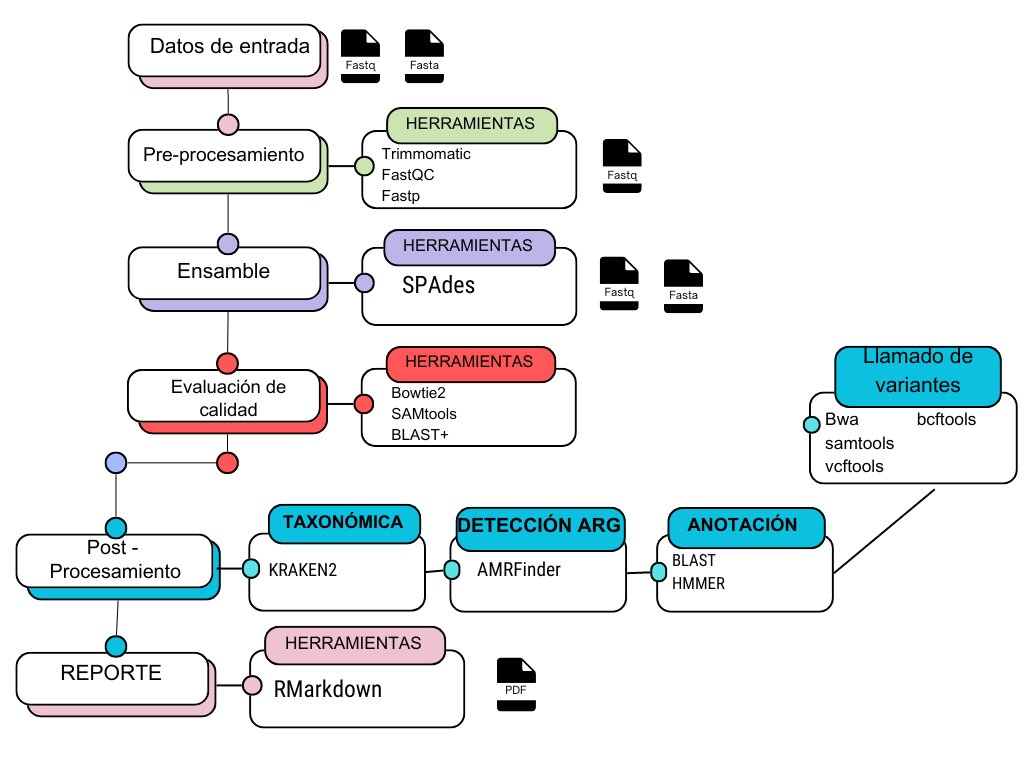
\includegraphics[scale=0.35]{seleccionMetodosAnalisis.png}
    \caption{Selección de herramientas y definición de los procesos del flujo de trabajo (\emph{elaboración propia}).} 
    \label{fig:seleccionMetodosAnalisis}
\end{figure}

En la figura \ref{fig:seleccionMetodosAnalisis} se puede 
observar cada etapa que será parte del flujo de trabajo. 
A continuación se definen las características generales  y 
utilidad  de cada una de ellas:

\begin{itemize}
    \item \textbf{Datos de entrada:} En esta etapa, el flujo de trabajo tendrá la capacidad de detectar y validar el formato entregado por el usuario. Es decir, si el usuario entrega un directorio que presente archivos variados como .csv .fasta .fq o bien .fq.gz, solo admitirá los que presenten .fasta .fq o .fq.gz.
    \item \textbf{Pre-procesamiento:} Para la etapa de pre-procesamiento, el usuario puede ejecutar el programa que prefiera en los archivos de entrada previos.  De esta manera, podrá limpiar, recortar o filtrar las lecturas antes de un ensamble o alineamiento o por el contrario, visualizar la calidad de las lecturas.
    \item \textbf{Ensamble o alineamiento:} Esta etapa permite  ensamblar o alinear las lecturas de entrada de usuario. Este podrá recibir las lecturas previamente pre-procesadas o bien, recibir las lecturas directamente de un archivo de entrada.
    \item \textbf{Evaluación de calidad:} La evaluación de calidad, ofrecerá al usuario la posibilidad de tener en una carpeta de trabajo de Nextflow,  todos los archivos de salida que se obtuvieron al calcular la calidad del ensamble o alineamiento.
    \item \textbf{Post-procesamiento:} La etapa de post-procesamiento, le otorga al usuario la opción de seleccionar, qué tipo de análisis quiere llevar a cabo en la cantidad disponible, Dentro de la tipología de análisis, el usuario puede considerar los siguientes:

        \begin{itemize}
            \item Análisis taxonómico
            \item Detección de genes de resistencia antibiótica
            \item Anotación funcional
            \item Llamado de variantes
        \end{itemize}
    
    \item \textbf{Reporte:} Finalmente, la característica del reporte, no es una opción que el usuario pueda desactivar o activar. Asimismo, este ofrecerá al usuario la información resumida de todos los procesos ejecutados dentro del flujo de trabajo, ya sea, pre-procesamiento, ensamble o alineamiento o cualquier análisis.
\end{itemize}

\subsection{Diseño e implementación del flujo de trabajo}

\begin{figure}[ht!]
    \centering
    \small
    \includegraphics[scale=0.35]{diseñoDelFlujoDeTrabajo.png}
    \caption{Diseño del flujo de trabajo (\emph{elaboración propia}).} 
    \label{fig:disenoDelFlujoDeTrabajo}
\end{figure}

Como se puede observar en la Fig.\ref{fig:disenoDelFlujoDeTrabajo} el flujo de trabajo 
consta de subflujos que determinan cómo los datos de entrada 
hacen variar la cantidad de procesos que se ejecutan.

El primer proceso que se puede observar es el proceso 
integral de análisis genómico de bacterias, en donde a partir 
del parámetro de entrada o dato de entrada, variará el flujo de 
trabajo.

La descarga inicia descrita en la Fig.\ref{fig:disenoDelFlujoDeTrabajo}, 
en el caso de que el usuario presente un directorio vacío 
acompañado de un código SRR \emph{(Sequence Read Archive Run)}, 
\emph{(que es un identificador único que se asigna a un conjunto 
específico de lecturas)}, podrá descargar desde NCBI las 
muestras. Al usuario, se le brinda la posibilidad de utilizar 
varios parámetros, es aquí, donde se encuentra \texttt{--path} que 
determina el directorio vacío, y en donde las lecturas
descargadas serán almacenadas. En el caso de \texttt{--id\_sra},
hace referencia al identificador de la lectura, que acompañado 
con el \texttt{--x} determinará la cantidad de lecturas a descargar. Si 
las lecturas presentan una librería Layout: PAIRED, se hace 
imprescindible la utilización de \texttt{--paires}.

\begin{center}
    \begin{lstlisting}[language=bash, caption=Sub-flujo de trabajo para la descarga inicial de lecturas \emph{(elaboración propia)}., label=lst:descargaInicial]
        nextflow run script.nf --path [directorio] \
            --id_sra [SRRXXXXXX] --x [lectura] --paires
    \end{lstlisting}
\end{center}

El flujo integral de análisis genómico de bacterias 
descrito en la Fig.\ref{fig:disenoDelFlujoDeTrabajo} permite 
que el usuario, al presentar un directorio que no esté vacío,  
almacene en un canal de trabajo 
de Nextflow, particularmente aquellos archivos que presenten la 
extensión de .fq, .fasta o .fq.gz o .fasta.gz. Cabe mencionar que, 
cualquier archivo que esté comprimido será descomprimido. El primer 
paso que puede activar el usuario, es la etapa de preprocesamiento, 
aquí el usuario puede utilizar herramientas como Fastqc o Trimmomatic. 
En el caso de utilizar Fastqc en todos los archivos dentro del 
directorio de entrada, la salida será una carpeta comprimida. La 
utilización de este programa limita las acciones que puede realizar 
el usuario, ya que no tiene una entrada válida para otro programa, 
tal como se puede observar en el List.\ref{lst:preprocesamientoFastqc}

\begin{center}
    \begin{lstlisting}[language=bash, caption=Comando para el preprocesamiento de las lecturas con Fastqc \emph{(elaboración propia)}., label=lst:preprocesamientoFastqc]
        nextflow run script.nf --path [directorio] \
            --fastqc
    \end{lstlisting}
\end{center}

Es importante remarcar que, una de las  herramienta que 
se complementa muy bien con las demás, es Trimmomatic. 
Esta herramienta, situándose dentro del grupo de trabajo, 
se le pueden utilizar las principales características del 
programa como tal, y como consecuencia, el archivo de salida 
será  apto para poder ensamblarse o alinearse, de acuerdo a  
como lo prefiera el usuario.

\newpage

\begin{center}
    \begin{lstlisting}[language=bash, caption=Comando de ejecución de etapa de pre procesamiento \emph{(elaboración propia)}., label=lst:preprocesamientoTrimmomatic]
        nextflow run script.nf --path [directorio de entrada]  \
            --trimmo [se o pe] \
            --threads [num de hilos] \
            --leading [valor de calidad para el recorte inicial] \
            --trailing [valor de calidad para el recorte final] \
            --slidingwindow [tamano de ventana: calidad min] \
            --minlen [longitud min. de lectura]
    \end{lstlisting}
\end{center}

En el List.\ref{lst:preprocesamientoTrimmomatic} se presentan 
los diferentes parámetros admitidos dentro del flujo de trabajo 
para una utilización de Trimmomatic, estos variarán de acuerdo a 
los requerimientos de cada usuario y de sus datos. La salida de 
este proceso es admitida para un ensamble o alineamiento.

La entrada para el proceso de ensamble o alineamiento, puede 
venir de un proceso previo, como fue descrito anteriormente, o bien, 
puede ser, a través de un archivo directo, entregado por el 
usuario \emph{(como se explica en la Fig.
\ref{fig:disenoDelFlujoDeTrabajo} en el análisis 
rápido de bacterias)}. De esta manera, la salida de este 
proceso permitirá la utilización de los diferentes análisis 
disponibles. 

De acuerdo a lo anterior, los análisis disponibles, 
vendrán  a complementar el proceso de ensamble y alineamiento, 
para así contar con  una mayor claridad con respecto a las muestras. 
Estos análisis, corresponden al análisis de detección de genes 
de resistencia antibiótica, análisis taxonómico, una anotación 
funcional y finalmente un llamado de variantes. Todos los análisis 
pueden ser usados, a través de la salida del ensamble o 
alineamiento, o bien a través de la entrada directa de una 
muestra (ver la Fig.\ref{fig:disenoDelFlujoDeTrabajo} en 
el análisis rápido de bacterias). 

El primer análisis que se puede describir, en razón de su 
utilización dentro del flujo de trabajo, corresponde al 
análisis de detección de genes de resistencia antibiótica. 
Este análisis, permite identificar y caracterizar genes de 
resistencia a antibióticos en secuencias genómicas. Su 
utilización, a través del flujo de trabajo se puede observar 
en la List.\ref{lst:argFast} y  List.\ref{lst:ARG}, 
con un análisis rápido o un análisis 
integral genómico de bacterias respectivamente. 

\newpage

\begin{center}
    \begin{lstlisting}[language=bash, caption=Comando para ejecutar un análisis rápido de identificación de genes de resistencia antibiótica \emph{(elaboración propia)}., label=lst:argFast]
        nextflow run script.nf --f [archivo de muestras]  \
            --arg [activar ARG] \
            --dbarg [base de datos de anotacion]
    \end{lstlisting}
\end{center}


\begin{center}
    \begin{lstlisting}[language=bash, caption=Comando para la ejecución de un análisis de ARG \emph{(elaboración propia)}., label=lst:ARG]
        nextflow run script.nf --path [directorio de entrada]  \
            --trimmo [se o pe] \
            --threads [num de hilos] \
            --leading [valor de calidad para el recorte inicial] \
            --trailing [valor de calidad para el recorte final] \
            --slidingwindow [tamano de ventana: calidad min] \
            --minlen [longitud min. de lectura] \
            --arg [activar ARG] \
            --dbarg [base de datos de anotacion]
    \end{lstlisting}
\end{center}

En el List.\ref{lst:ARG} se puede observar cómo se implementan los 
procesos de preprocesamiento y ensamble, junto al análisis 
de detección de genes de resistencia antibiótica. En esta 
etapa, sólo se necesita para activar el proceso, la bandera 
\texttt{--arg} y para seleccionar la base de datos para la anotación 
\texttt{--dbarg}. Cabe destacar, que esto no impide que otros análisis 
sean activados por el usuario.

En el caso del análisis taxonómico, se refiere a la 
identificación de los organismos presentes en una muestra, 
a partir de sus secuencias de ADN o ARN. 

\begin{center}
    \begin{lstlisting}[language=bash, caption=Comando para ejecutar un análisis rápido de identificación taxonómica \emph{(elaboración propia)}., label=lst:taxonomyFast]
        nextflow run script.nf --f [archivo de muestras]  \
            --taxonomy [activar opc] \
            --db [ruta a la base de datos]
    \end{lstlisting}
\end{center}


\begin{center}
    \begin{lstlisting}[language=bash, caption=Comando para la ejecución de un análisis de identificación taxonómica \emph{(elaboración propia)}., label=lst:TAXONOMY]
        nextflow run script.nf --path [directorio de entrada]  \
            --trimmo [se o pe] \
            --threads [num de hilos] \
            --leading [valor de calidad para el recorte inicial] \
            --trailing [valor de calidad para el recorte final] \
            --slidingwindow [tamano de ventana: calidad min] \
            --minlen [longitud min. de lectura] \
            --taxonomy [activar opc] \
            --db [ruta a la base de datos]
    \end{lstlisting}
\end{center}

En el List.\ref{lst:taxonomyFast} y List.\ref{lst:TAXONOMY} se puede 
observar, cómo utilizar este análisis, a través del flujo de 
trabajo, en un análisis rápido o en un análisis más completo. 
El usuario para activar la opción debe utilizar \texttt{--taxonomy}, y 
además ingresar con \texttt{--db} la ruta a la base de datos que desee  
utilizar.

Un llamado de variantes, es poder identificar diferencias genéticas, 
como SNPs, pequeñas inserciones o deleciones \emph{(indels)}, comparando 
las secuencias de una muestra con una referencia. En este caso, el 
usuario podrá utilizar como muestra el resultado del ensamble o 
alineamiento (ver List.\ref{lst:VARIANTES}) o bien, puede optar por  ingresar un 
archivo .fasta para la comparación. Sin embargo, con eso no basta, 
el debe ingresar un genoma de referencia, a través del parámetro 
\texttt{--variantRef}. Si por alguna razón, no presenta un genoma de 
referencia pero sí presenta un identificador NC de NCBI, lo 
podrá realizar, a través del parámetro \texttt{--variantRefId}.

\begin{center}
    \begin{lstlisting}[language=bash, caption=Comando para ejecutar un análisis rápido de llamado de variantes \emph{(elaboración propia)}., label=lst:variantesFast]
        nextflow run script.nf --f [archivo de muestras]  \
            --variantCall [activar opc] \
            --variantRef [ruta del genoma de referencia]
    \end{lstlisting}
\end{center}

\begin{center}
    \begin{lstlisting}[language=bash, caption=Comando para la ejecución de un análisis de llamado de variantes \emph{(elaboración propia)}., label=lst:VARIANTES]
        nextflow run script.nf --path [directorio de entrada]  \
            --trimmo [se o pe] \
            --threads [num de hilos] \
            --leading [valor de calidad para el recorte inicial] \
            --trailing [valor de calidad para el recorte final] \
            --slidingwindow [tamano de ventana: calidad min] \
            --minlen [longitud min. de lectura] \
            --variantCall [activar opc] \
            --variantRef [ruta del genoma de referencia]
    \end{lstlisting}
\end{center}

El último análisis disponible, dentro del flujo de trabajo, 
corresponde a  la anotación funcional, que se refiere al 
proceso de asignar, anotar funciones biológicas a las secuencias, 
como genes o variantes. En este mismo contexto, el usuario podrá 
activar esta opción con el parámetro \texttt{--annotation} y entregando la
ruta al archivo para generar la base de datos con \texttt{--ref annotation}.

\begin{center}
    \begin{lstlisting}[language=bash, caption=Comando para ejecutar un análisis rápido de anotación funcional \emph{(elaboración propia)}., label=lst:annotationFast]
        nextflow run script.nf --f [archivo de muestras]  \
            --annotation [activar opc] \
            --refannotation [archivo para crear base de datos]
    \end{lstlisting}
\end{center}

\begin{center}
    \begin{lstlisting}[language=bash, caption=Comando para la ejecución de una anotación funcional \emph{(elaboración propia)}., label=lst:ANNOTATION]
        nextflow run script.nf --path [directorio de entrada]  \
            --trimmo [se o pe] \
            --threads [num de hilos] \
            --leading [valor de calidad para el recorte inicial] \
            --trailing [valor de calidad para el recorte final] \
            --slidingwindow [tamano de ventana: calidad min] \
            --minlen [longitud min. de lectura] \
            --annotation [activar opc] \
            --refannotation [archivo para crear base de datos]
    \end{lstlisting}
\end{center}

Por último, se debe indicar que cada proceso ejecutado durante el flujo de trabajo, 
tiene su propio ambiente, que corresponde a una carpeta o directorio dentro de una 
asignada por Nextflow. En este caso, nos referimos a la carpeta works, aquí se podrán 
encontrar todas las salidas de las herramientas utilizadas y los links o rutas 
simbólicas a los archivos de entrada.

\subsection{Casos de estudio}

En este capítulo, se presentarán diferentes casos de estudio para representar una 
ejecución del flujo de trabajo en un ambiente investigativo. Esto se realizará por 
cada análisis por separado, de modo de verificar y controlar los resultados.

\subsubsection*{Caracterización de Genes de Resistencia Antibiótica y Clasificación 
Taxonómica en \textit{Escherichia coli}}

El primer caso corresponde a la evaluación de la 
\textit{Escherichia coli} \emph{(E. coli)}, comúnmente encontrada en el 
intestino del humano y otros animales. La mayoría de las cepas de 
E. coli son inofensivas, sin embargo, algunas cepas pueden causar 
infecciones graves, como diarrea, o enfermedades respiratorias. 
En este contexto, la evaluación o detección de genes de resistencia 
antibiótica es crucial, debido a su capacidad de adquirir o transferir 
resistencia, representando un desafío significativo para la salud 
pública.

En primer lugar, una vez realizada la búsqueda en NCBI SRA, para 
identificar un SRR de \textit{Escherichia coli} \emph{(E. coli)} 
válido, se usará la descarga inicial del flujo de trabajo, 
como se muestra en el List.\ref{lst:descargaCaso1}.

\begin{center}
    \begin{lstlisting}[language=bash, caption=Comando para la descarga inicial de las muestras de \textit{Escherichia coli} \emph{(elaboración propia)}., label=lst:descargaCaso1]
        nextflow run script.nf --path [directorio]  \
            --id_sra SRR291523311 \
            --x 500 \
            --pairs
    \end{lstlisting}
\end{center}

En el List.\ref{lst:descargaCaso1}, se puede apreciar la utilización de parámetros 
como es el caso de \texttt{--path}, que puede ser cualquier directorio 
vacío, \texttt{--id\_sra} que 
se le entrega el código SRR de NCBI,  en donde, las muestras presentan una librería PAIRED, 
por lo que se hace imprescindible la utilización de \texttt{--pairs} y la cantidad de 
lecturas a 
descargar, que en este caso solo serán las primeras 500. Una vez obtenidas las lecturas a 
utilizar de  \textit{Escherichia coli} \emph{(E. coli)}, se utilizara el 
flujo de trabajo que lleva 
por nombre, \emph{“proceso integral de análisis de bacterias”} para poder realizar un 
preprocesamiento, un ensamble y un análisis de detección de genes de resistencia 
antibiótica. De esta manera, los parámetros utilizados se pueden observar en la figura 
que a continuación se presenta:

\begin{center}
    \begin{lstlisting}[language=bash, caption=Comando para la identificación de ARG de \textit{Escherichia coli} \emph{(elaboración propia)}., label=lst:ARGCaso1]
        nextflow run script.nf --path misc/mocks \
            --trimmo pe \
            --threads 3 \
            --leading 3 \
            --trailing 3 \
            --minlen 36 \
            --spades \ 
            --arg \
            --typedb plasmidfinder
    \end{lstlisting}
\end{center}

Para la realización de este análisis, el preprocesamiento de las lecturas se 
ejecutó en base a un filtrado, en donde el valor de calidad para recorte 
inicial \emph{(leading)} tiene un valor de 3, el valor de calidad para el recorte 
final \emph{(trailing)} será de 3 y  la longitud mínima de lectura \emph{(minlen)}
tendrá un valor de  36. De esta manera, el ensamble de novo se debería 
realizar de manera exitosa, permitiendo la utilización de la base de datos 
plasmidfinder para detectar genes de resistencia antibiótica.

Los resultados de la detección de genes de resistencia antibiótica 
identificaron la presencia del gen Col(BS512)\_1 en la secuencia, con
una cobertura del 87.98\% y una identidad del 99.51\%. Este gen, 
está registrado en la base de datos plasmidfinder bajo el acceso NC\_010656.

A modo de, sintetizar la etapa de casos de uso, y brindar un mayor 
entendimiento del cómo funcionan los análisis dentro del flujo de 
trabajo, el  análisis taxonómico se realizará en base a la misma 
muestra de \textit{Escherichia coli} \emph{(E. coli)}. De esta manera, si se entrega 
directamente una muestra de \textit{Escherichia coli} a Kraken 2, el software 
intentará clasificar de acuerdo a su base de datos taxonómica predefinida 
para identificar el organismo al que pertenece. En este caso, al tratarse 
de \textit{Escherichia coli}, Kraken 2 debería clasificar correctamente la secuencia 
como perteneciente a esa especie bacteriana. 

De esta manera, se realizó un análisis taxonómico de una muestra de 
\textit{Escherichia coli} utilizando la herramienta kraken 2. El objetivo es 
identificar la composición taxonómica de la muestra y determinar si 
presenta elementos virales.

Para la ejecución del flujo de trabajo, se debe descargar la 
base de datos de kraken 2 para determinar la presencia de elementos 
virales, utilizando el parámetro \texttt{--dbdownload} y el nombre de la base 
de datos que es \emph{Viral}. De esta manera, se puede continuar con la 
ejecución del flujo de trabajo, con los parámetros que se pueden ver 
en el List.\ref{lst:TAXONOMYCaso1}:


\begin{center}
    \begin{lstlisting}[language=bash, caption=Comando para la identificación taxonómica de \textit{Escherichia coli} \emph{(elaboración propia)}., label=lst:TAXONOMYCaso1]
        nextflow run script.nf --path misc/mocks \
            --trimmo pe \
            --threads 3 \
            --leading 3 \
            --trailing 3 \
            --minlen 36 \
            --spades \ 
            --taxonomy \
            --db [base de datos viral]
    \end{lstlisting}
\end{center}


Entonces, se utilizó una base de datos viral de Kraken 2 que 
incluye secuencias de diversos organismos, y la ejecución del 
comando del List.\ref{lst:TAXONOMYCaso1}, los resultados 
se pueden ver en anexos.

Se detectaron secuencias no clasificadas, que pueden deberse a 
secuencias de baja calidad, incompletas o que no tienen 
coincidencias en la base de datos utilizada, que corresponden 
al 94.87\% (37 secuencias). Al mismo tiempo, el  5.13\% de las 
secuencias, fueron clasificadas como virus pertenecientes 
al reino Duplodnaviria. Además, se detectó la presencia 
de Escherichia phage 500465\-1 y Escherichia phage ev099, 
qué son los fagos que infectan \textit{Escherichia coli}.

Para concluir sobre este caso de estudio, el análisis 
taxonómico realizado con el flujo de trabajo, permitió 
identificar una pequeña muestra de secuencias virales que 
infectan \textit{Escherichia coli}. Sin embargo, la alta 
cantidad de secuencias 
no clasificadas demuestra que hay una necesidad de mejorar 
la calidad de las lecturas o bien, cambiar la base de datos.

\subsubsection*{Análisis Funcional y Bioinformático de 
Beta-Galactosidasa en \textit{Escherichia coli}}

En cuanto al caso de estudio siguiente, lo que se realizará, 
es un análisis funcional de Beta-Galactosidasa de 
\textit{Escherichia coli}, utilizando el flujo de trabajo. 
Cabe mencionar que la beta-galactosidasa, es una enzima 
producida por la bacteria que cataliza la hidrólisis de la 
lactosa en glucosa y galactosa.

En primer término, se obtuvieron todas las secuencias de 
beta-galactosidasa de \textit{Escherichia coli} desde 
la base de datos 
UniProt en formato FASTA, luego se buscó \emph{“Escherichia 
coli beta-galactosidase”}, en la base de datos NCBI 
Nucleotide y se descargó la secuencia de nucleótidos 
correspondiente en formato FASTA. Finalmente, era necesario 
identificar todos los ORFs \emph{(Open Reading Frames)} en la secuencia 
obtenida de NCBI Nucleotide, usando la herramienta ORF finder. 
De esta manera, el flujo tendría todo lo necesario para 
ejecutar el análisis con el comando, tal como señala 
el List.\ref{lst:ANNOTATIONCaso1}:

\begin{center}
    \begin{lstlisting}[language=bash, caption=Comando para la anotación funcional de \textit{Escherichia coli} \emph{(elaboración propia)}., label=lst:ANNOTATIONCaso1]
        nextflow run script.nf --f ORF.fa \
        --annotation \
        --annotationDb database.fa \
        --annotationType prot
    \end{lstlisting}
\end{center}

Los resultados de la anotación funcional de los ORFs, que se encuentran en la 
tabla de anexos, arrojan que de los siete ORFs en la secuencia 
de ADN de \emph{E. coli}, 
ninguno de los ORFs mostró coincidencias significativas en 
la base de datos utilizada. 
Lo anterior, puede deberse a varias razones, entre ellas, que 
la base de datos 
BLAST utilizada, podría no presentar secuencias correspondientes 
o bien, los ORFs 
podrían ser regiones no codificantes o no estar anotadas previamente. 
Sin embargo, 
aunque no se obtuvieron los resultados esperados, si se puede tener el 
alcance de la 
funcionalidad del flujo de trabajo.

\subsubsection*{Análisis de Variantes Genéticas en Escherichia coli Mediante 
el Genoma de Referencia ASM584v2}

Para el siguiente caso de estudio y para validar la implementación de la 
llamada de variantes se descargará el genoma de referencia \emph{ASM584v2} de 
\textit{Escherichia coli} para identificar variantes genéticas. A continuación se mostrará 
el comando ejecutado:

\begin{center}
    \begin{lstlisting}[language=bash, caption=Comando para realizar un llama de variantes en \textit{Escherichia coli} \emph{(elaboración propia)}., label=lst:VARIANTCaso1]
        nextflow run script.nf --path misc/mocks/ \
        --trimmo pe \
        --threads 3 \
        --leading 3 \
        --trailing 3 \
        --minlen 3 \
        --spades \
        --variantCall \
        --variantRef GCA_000005845.2_ASM584v2_genomic.fna 
    \end{lstlisting}
\end{center}

Considerando que el \emph{variant calling} es 
crucial para entender las diferencias genéticas y 
su impacto funcional. Este proceso es la base de
muchos estudios genómicos y tiene aplicaciones 
directas en medicina, de esta manera, se detectaron 
90 SNPs en la muestra analizada, también el ratio 
de transiciones a transversiones \emph{(ts/tv)} 
fue de 2.10, 
que es un indicador de la calidad del llamado de 
variantes. 

La implementación del flujo de trabajo, y con 
ello de las herramientas que llevan a cabo los 
diferentes análisis, fue generado en un ambiente 
controlado, que posteriormente, tendrá que empaquetarse 
para garantizar su reproducibilidad, junto además, 
a la generación de una documentación.

\subsection{Diseño y estructura de los reportes}

La definición del diseño y estructura de los 
reportes, se basa en primer lugar en encontrar 
la manera de entregarle al usuario la información 
precisa o resumida sobre un análisis o proceso 
realizado.

\subsection{Implementación de los reportes}

La implementación de los reportes, planteó un desafío ya que Nextflow 
no maneja eventos posteriores al  flujo de trabajo principal haya terminado. 
Por otro lado, Nextflow tiene su propia manera de manejar los archivos de 
salida de cada proceso, almacenando los archivos de salida con un 
identificador dinámico difícil de manejar.

De esta manera, era necesario generar una forma de determinar el 
momento exacto que los archivos de salida asíncronos de los procesos 
ejecutados por el usuario haya terminado para finalmente utilizarlos para 
generar un reporte.

La estrategia utilizada para determinar, qué procesos fueron 
seleccionados por el usuario, y de esta forma el reporte tenga 
una estructura dinámica fue generar una dependencia a un canal de 
cola, una funcionalidad propia de Nextflow. Esto permite, que el 
código intérprete que debe esperar que el canal reciba un valor para 
continuar con el proceso del informe.

Así, si los parámetros trimmo y spades están presentes, se evaluarán 
diferentes combinaciones de los parámetros taxonomy, arg, annotation y 
variantCall para determinar qué acciones tomar y qué resultados visualizar.
La siguiente tabla detalla las combinaciones posibles y las acciones 
correspondientes. 

\begin{longtable}{|c|c|c|c|p{6cm}|}
    \caption{Estrategía utilizada para la implementación de los reportes con sus respectivas acciones (elaboración propia).}
    \label{tabla:acciones} \\
    \hline
    \textbf{Taxonomy} & \textbf{ARG} & \textbf{Annotation} & \textbf{VariantCall} & \textbf{Acción} \\
    \hline
    \endfirsthead
    
    \hline
    \textbf{Taxonomy} & \textbf{ARG} & \textbf{Annotation} & \textbf{VariantCall} & \textbf{Acción} \\
    \hline
    \endhead
    
    \hline \multicolumn{5}{r}{\textit{Continúa en la siguiente página}} \\
    \endfoot
    
    \hline
    \endlastfoot
    
    False & False & False & False & Visualizar solo el resultado de Spades \\
    \hline
    False & False & False & True & Visualizar el resultado de Variant Calling \\
    \hline
    False & False & True & False & Visualizar el resultado de Annotation \\
    \hline
    False & False & True & True & Visualizar los resultados de Annotation y Variant Calling \\
    \hline
    False & True & False & False & Visualizar el resultado de ARG \\
    \hline
    False & True & False & True & Visualizar los resultados de ARG y Variant Calling \\
    \hline
    False & True & True & False & Visualizar los resultados de ARG y Annotation \\
    \hline
    False & True & True & True & Visualizar los resultados de ARG, Annotation, y Variant Calling \\
    \hline
    True & False & False & False & Visualizar el resultado de Taxonomy \\
    \hline
    True & False & False & True & Visualizar los resultados de Taxonomy y Variant Calling \\
    \hline
    True & False & True & False & Visualizar los resultados de Taxonomy y Annotation \\
    \hline
    True & False & True & True & Visualizar los resultados de Taxonomy, Annotation, y Variant Calling \\
    \hline
    True & True & False & False & Visualizar los resultados de Taxonomy y ARG \\
    \hline
    True & True & False & True & Visualizar los resultados de Taxonomy, ARG, y Variant Calling \\
    \hline
    True & True & True & False & Visualizar los resultados de Taxonomy, ARG y Annotation \\
    \hline
    True & True & True & True & Visualizar todos los resultados \\
    \hline
\end{longtable}

Destacar, que esta fue la estrategia para el flujo de 
trabajo con ensamble o alineamiento, o para un análisis 
rápido de bacterias.

\subsection{Documentación del flujo de trabajo}

El flujo de trabajo está alojado dentro de un repositorio de 
GitHub, 
este sigue una estructura sencilla de organización que 
se puede ver en la figura a continuación.

\begin{figure}[htbp]
    \centering
    \begin{forest}
        for tree={
            font=\ttfamily,  % Fuente de tipo de letra tipo teletipo
            grow=east,       % Crece hacia la derecha
            align=left,      % Alineación a la izquierda
            anchor=west,     % Ancla en el oeste (izquierda)
            child anchor=west, % Ancla los hijos al oeste
            edge path={
                \noexpand\path [draw, \forestoption{edge}]
                (!u.south east) -- ++(5pt,0) |- (.child anchor)\forestoption{edge label};
            },
            l sep=15pt, % Espaciado vertical entre nodos
            s sep=10pt, % Espaciado horizontal entre nodos
            parent anchor=east % Ancla los padres al este (derecha)
        }
        [repositorio de trabajo % Nodo raíz
            [config % Carpeta config
                [Dockerfile]
            ]
            [.gitignore]  % Archivos en el directorio raíz
            [misc]  % Carpeta misc
            [src % Carpeta src
                [process]  % Subcarpetas dentro de src
                [workflows]
                [services]
            ]
            [README.md]
            [docker-compose.yml]
            [nextflow.config]
            [script.nf]
        ]
    \end{forest}
    \caption{Estructura del repositorio de trabajo.}
    \label{fig:repositorio}
\end{figure}

Es una estructura sencilla en donde en el directorio 
config, se contienen todos los archivos de configuración 
específicos, en este caso el Dockerfile. En el caso 
del directorio misc, es un directorio misceláneo que 
solo se utiliza para archivos que puedan ser necesarios, 
como las muestras utilizadas en los casos de estudio. El 
directorio principal que contiene el código fuente 
del proyecto es el nombrado src, este presenta otros 
tres directorios que son process, que contiene las 
definiciones de todos los procesos utilizados en el flujo, 
el directorio workflow que define todos los subflujos de 
trabajo del pipeline, y finalmente services, que son todas 
las utilidades y validaciones necesarias para el correcto 
funcionamiento del flujo. Además de la carpeta principal src, 
se tienen archivos en la raíz del proyecto como el gitignore, 
que especifica los archivos o directorios ignorados por el 
git, el archivo README que describe la documentación del 
proyecto,  el archivo docker-compose.yml que es el archivo 
de configuración del servicio de docker, el nextflow.config, 
que es el archivo de configuración de Nextflow, contiene 
parámetros y ajustes de memoria, y finalmente el script.nf 
que es el archivo que define el flujo de trabajo.

La documentación del flujo de trabajo, se llevó a cabo en el 
archivo README, y  presenta un encabezado con el título 
del proyecto y varias insignias que indican la versión, 
estado de construcción, cobertura de código y licencia. 
La Introducción explica el propósito del pipeline 
desarrollado en NextFlow para el análisis de bacterias, 
destacando su accesibilidad y automatización. La sección 
de Instalación y Configuración proporciona instrucciones 
para clonar el repositorio, instalar Docker Desktop y 
generar la imagen Docker necesaria. Las Instrucciones de 
Uso detallan los pasos para comenzar a usar el pipeline, 
incluyendo la configuración de directorios y parámetros 
específicos. La sección de Preprocesamiento describe el 
uso de herramientas como FastQC y Trimmomatic para procesar 
las lecturas de secuenciación antes del análisis. 
En Ensamble, se explica cómo ensamblar genomas 
bacterianos utilizando SPAdes, incluyendo opciones 
para preprocesamiento y ensamblaje conjunto. La sección 
de Análisis incluye sub-secciones sobre la 
identificación taxonómica usando Kraken 2, la 
identificación de genes de resistencia a antibióticos 
usando AMRFinder, el llamado de variantes genéticas, y 
la anotación funcional de secuencias ensambladas. 
Un Ejemplo de Uso proporciona un ejemplo de ejecución 
del pipeline que combina varios análisis a partir de 
un directorio con datos de trabajo. La sección de 
Reporte informa sobre la generación de un informe 
resumen en formato PDF con los resultados del pipeline, 
destacando la disponibilidad de output detallado en la 
carpeta work. Configuración Avanzada ofrece instrucciones 
para configurar directorios de trabajo y otros parámetros 
en el archivo nextflow.config. La sección sobre Detalles 
sobre las versiones específicas de las herramientas 
utilizadas lista todas las dependencias y requisitos de 
software utilizados en el proyecto. Solución de Problemas 
proporciona consejos para resolver problemas comunes en 
los procesos de ensamblaje, anotación y taxonomía. 
Finalmente, la sección de Licencia informa sobre la 
licencia MIT bajo la cual se distribuye el proyecto. 

\subsection{Empaquetamiento del flujo de trabajo}

Para el empaquetamiento del flujo de trabajo, se 
utilizó la herramienta de docker, que permite la 
automatización del despliegue de aplicaciones dentro de  
contenedores. En nuestro caso, se seleccionó una imagen 
base de Ubuntu para construir el contenedor. Esta se 
seleccionó, ya que es una opción estándar debido a su 
estabilidad y amplia compatibilidad con diversas herramientas, 
bibliotecas y dependencias, es decir, garantizamos un 
entorno reproducible y portátil.

Para integrar Docker con Nextflow y escalar el 
flujo de trabajo, se configuró un servicio en el 
directorio de configuración del repositorio. Aquí se 
define cómo se construye el contenedor y cómo se montan 
los volúmenes para asegurar que los archivos de trabajo 
estén disponibles dentro del contenedor. Esta se puede ver 
en la figura \ref{lst:servicesDocker} siguiente.

\begin{center}
    \begin{lstlisting}[language=bash, caption=Código para la elaboración del servicio de docker \emph{(elaboración propia)}., label=lst:servicesDocker]
        services:
            pipeline:
                build:
                    context:
                    dockerfile: ./config/Dockerfile
                volumes:
                    - ${PWD}:/workspace
    \end{lstlisting}
\end{center}

En el List.\ref{lst:servicesDocker} se puede apreciar 
la configuración del archivo para generar el servicio, 
en este se aprecia la palabra reservada context, que 
vendría a ser el contexto de construcción, es decir, 
se refiere al directorio desde el cual Docker copiará 
los archivos a la imagen del contenedor. Al mismo tiempo, 
se visualiza la palabra reservada Dockerfile, que es la 
ruta al archivo Dockerfile que define cómo construir la 
imagen. Volumes, o en español volúmenes, monta el directorio 
de trabajo actual, dentro del contenedor, permitiendo tener 
acceso a los archivos del proyecto.

Dentro del archivo de configuración de docker, o 
dockerfile, se encuentran todas las dependencias  y 
herramientas vitales para la ejecución del flujo de 
trabajo, a continuación se nombrarán las herramientas 
instaladas dentro de la imagen de docker.


\begin{longtable}{|c|p{6cm}|}
    \caption{Información sobre las herramientas instaladas dentro de la imagen docker (elaboración propia).}
    \label{tabla:asasd} \\
    \hline
    \textbf{Herramienta / dependencia} & \textbf{Descripción}  \\
    \hline
    \endfirsthead
    
    \hline
    \textbf{Herramienta / dependencia} & \textbf{Descripción} \\
    \hline
    \endhead
    
    \hline \multicolumn{2}{r}{\textit{Continúa en la siguiente página}} \\
    \endfoot
    
    \hline
    \endlastfoot
    
    Ubuntu & Sistema operativo base utilizado en el contenedor \\
    \hline
    openjdk-11-jre-headless & Entorno de ejecución de Java necesario para ejecutar aplicaciones Java sin interfaz gráfica. \\
    \hline
    curl & Herramienta de línea de comandos para transferir datos con URL \\
    \hline
    unzip & Utilidad para descomprimir archivos .zip \\
    \hline
    trimmomatic & Herramienta para el recorte de secuencias de ADN \\
    \hline
    fastqc & Programa para el control de calidad de datos de secuencias de alto rendimiento \\
    \hline
    wget & Herramienta de línea de comandos para descargar archivos de la web \\
    \hline
    spades & Ensamblador de genomas de lectura corta, de novo. \\
    \hline
    python3 & Lenguaje de programación Python, versión 3.\\
    \hline
    build$-$essential & Conjunto de herramientas de desarrollo, incluyendo el compilador GCC y las bibliotecas necesarias \\
    \hline
    Nextflow & Framework para la creación y ejecución de flujos de trabajo bioinformáticos. \\
    \hline
    SRA Toolkit & Conjunto de herramientas para descargar y manejar datos de secuencias SRA de NCBI. \\
    \hline
    Bowtie2 & Alineador de secuencias para la lecturas de ADN cortas. \\
    \hline
    Kraken2 & Sistema de clasificación y análisis taxonómico de secuencias. \\
    \hline
    ncbi$-$blast$+$ & Herramientas para realizar búsquedas de alineamiento de secuencias. \\
    \hline
    HMMER & Software para la detección de homologías en secuencias biológicas. \\
    \hline
    R & Lenguaje de programación y entorno para análisis estadístico y gráficos. \\
    \hline
    libcurl4-openssl-dev & Biblioteca de desarrollo para \emph{curl} con soporte para OpenSSL. \\
    \hline
    libssl-dev & Biblioteca de desarrollo para OpenSSL, necesario para conexiones seguras. \\
    \hline
    libxml2-dev & Biblioteca de desarrollo para XML. \\
    \hline
    devtools (R) & Paquete de R para facilitar el desarrollo de paquetes de R. \\
    \hline
    XML (R) & Paquete de R para trabajar con datos XML. \\
    \hline
    rentrez & Paquete de R para interactuar con las bases de datos de NCBI. \\
    \hline
    autoconf & Herramienta para generar scripts de configuración automática. \\
    \hline
    git & Sistema de control de versiones. \\
    \hline
    VCFtools & Conjunto de herramientas para trabajar con archivos VCF (Variant Call Format). \\
    \hline
    BWA & Alineador de secuencias para lecturas cortas. \\
    \hline
    libvcflib-tools & Herramientas para manipular archivos VCF. \\
    \hline
    libvcflib-dev & Biblioteca de desarrollo para libvcflib-tools. \\
    \hline
    freebayes & Detector de variantes genéticas de múltiples muestras. \\
    \hline
    vcfR (R) & Paquete de R para la manipulación y análisis de archivos VCF. \\
    \hline
    bcftools & Conjunto de herramientas para trabajar con archivos VCF y BCF. \\
    \hline
    libdatetime-perl & Módulo de Perl para trabajar con fechas y horas. \\
    \hline
    libxml-simple-perl & Módulo de Perl para leer y escribir archivos XML. \\
    \hline
    libdigest-md5-perl & Módulo de Perl para crear resúmenes MD5. \\
    \hline
    default-jre & Entorno de ejecución de Java por defecto. \\
    \hline
    bioperl & Colección de módulos Perl para bioinformática. \\
    \hline
    Bio::Perl & Módulo de Perl para secuencias biológicas. \\
    \hline
    libidn11 & Biblioteca para el manejo de nombres de dominio internacionalizados. \\
    \hline
    gzip & Herramienta de compresión de archivos. \\
    \hline
    libjson-perl & Módulo de Perl para trabajar con datos JSON. \\
    \hline
    libtext-csv-perl & Módulo de Perl para manipular archivos CSV. \\
    \hline
    libpath-tiny-perl & Módulo de Perl para manipular rutas de archivos. \\
    \hline
    liblwp-protocol-https-perl & Módulo de Perl para hacer solicitudes HTTP seguras. \\
    \hline
    libwww-perl & Módulo de Perl para interactuar con la web. \\
    \hline
    cpanminus & Instalador de módulos Perl. \\
    \hline
    LWP::Simple (Perl) & Módulo de Perl para hacer solicitudes HTTP sencillas. \\
    \hline
    any2fasta & Herramienta para convertir secuencias biológicas a formato FASTA. \\
    \hline
    Abricate & Herramienta para la detección de elementos genéticos en secuencias. \\
    \hline
\end{longtable}

En el caso de la instalación de Nextflow, SRA Toolkit se instalaron descargando 
los scripts de instalación y moviéndose al directorio /usr/local/bin. En el caso de Bowtie2, 
Kraken 2 y Abricate, se descargaron desde GitHub, y se instalaron manualmente añadiendo el 
binario al path. Por otra parte, HMMER, VCFtools y BWA, se descargaron y se instalaron 
desde la fuente. Los módulos de BioPerl y Perl se instalaron usando cpan y cpanminus. Los 
diferentes paquetes de R y R, se instalaron devtools, XML, vcfR desde CRAN y rentrez desde 
Github.

De esta manera, se garantiza la capacidad del flujo de trabajo de ser portable y 
reproducible en diferentes ambientes, con el único requerimiento de tener Docker.

\newpage
\section{Discusión}
La búsqueda bibliográfica permitió identificar diferentes herramientas que permiten
 una correcta ejecución del flujo de trabajo del grupo seleccionado para la 
 identificación de genes de resistencia antibiótica, se tuvo dificultades para 
 instalar y ejecutar la gran mayoría de las opciones. La documentación, reflejaba 
 una instalación basada en contenedor, lo que dificulta la instalación del ejecutable 
 en nuestro propio ambiente de ejecución. Es por lo anterior, que se prefirió la utilización 
 de un software que utiliza las bases de datos para la comparación como Resfinder 
 o de NCBI para generar la identificación y anotación de los genes. 

El diseño del flujo de trabajo, no presenta la posibilidad de seleccionar la 
herramienta a usar para los análisis, si no que por el contrario, existen 
herramientas predefinidas, detrás de la activación de la funcionalidad del usuario. 
Aquí, nace la posibilidad  de evaluar si en futuras versiones, darle la 
cualidad al usuario de seleccionar la herramienta a usar por análisis mejoraría 
la usabilidad y rendimiento del flujo de trabajo. 

El diseño actual, presente en este trabajo brinda la posibilidad de 
ejecutar diferentes análisis, con el único objetivo de mejorar la automatización de 
diversas herramientas bioinformáticas, sin duda, el servicio de este flujo de trabajo 
puede ser un instrumento potencialmente favorable para su utilización en 
investigaciones. De lo anterior, nace la problemática de seguir mejorando la 
automatización, optimizando el código, encontrando nuevas funcionalidad que vayan 
escalando junto al lenguaje de Nextflow.

Dentro del flujo de trabajo se optó por agregar diferentes funcionalidades que le 
ofrezcan al usuario una mejor “calidad de vida” y una mayor automatización, como la 
descarga de genomas de referencia, la utilización de SRA Toolkit para la descarga de 
las muestras en formato .fastq, la posibilidad de descomprimir directamente los 
archivos desde el flujo de trabajo o como también la descarga de las bases de datos 
para el análisis taxonómico. Sin duda, ninguna de estas funcionalidades intenta 
aumentar el tamaño de la imágen de docker, o disminuir el rendimiento, se tendrá que 
evaluar la usabilidad de cada una de estas características.

Una de las funcionalidades más importantes, es la implementación de un reporte 
final automatizado, que brinda la posibilidad al usuario de obtener la información 
de los procesos ejecutados de manera resumida. Sin duda, la implementación marcó un 
desafío, ya que, el lenguaje base del flujo de trabajo está escrito en Nextflow. Este 
lenguaje no brinda la funcionalidad de ejecutar otro proceso terminado el flujo de 
trabajo principal, que serían todos los procesos seleccionados por el usuario. De esta 
manera, se tuvo que generar un canal para generar una dependencia y que reciba los 
resultados de cada proceso ejecutado y así detectar el momento en que los procesos del 
“flujo principal” terminen. Esta manera de detectar cuándo ejecutar el proceso que 
realiza el informe, sin duda, marca una lentitud en el rendimiento general y puede 
ser mejorada con alguna actualización de Nextflow futura.

	
La ejecución de los casos de estudios, se realizaron bajo un ambiente de bajo 
rendimiento, en un computador con 7 GB de RAM lo cual limitó nuestra capacidad 
de procesamiento de datos. Las restricciones de memoria afectaron significativamente 
la capacidad para ejecutar herramientas bioinformáticas intensivas en recursos como 
Kraken 2 y Spades de manera eficiente. Para manejar estas limitaciones, utilizamos 
varias estrategias. Ocupamos versiones más ligeras de las bases de datos y ejecutamos 
los análisis en fragmentos más pequeños de datos en lugar de analizar muestras 
completas de una vez. Lo cual, se puede observar, en la base de datos utilizada en 
el proceso de identificación taxonómica donde se utilizó la colección de muestras 
virales de un tamaño de 0.5 GB . Otro ejemplo claro, es la utilización de las primeras 
500 lecturas de escherichia coli y no el genoma de la muestra completo. Además, 
se implementaron técnicas de optimización de memoria, como la liberación de caché y el 
uso de datos comprimidos que permitieron completar los análisis, pero también presentaron 
desafíos, como tiempos de ejecución prolongados y la necesidad de realizar múltiples 
repeticiones para verificar los resultados. Es por esto, que para futuros usos, 
se recomienda el uso de sistemas con mayor capacidad de memoria acelerando los tiempos 
de análisis,y brindando la opción de usar datos de entrada más grandes. Es decir, las 
limitaciones de hardware presentaron desafíos significativos, y que si no es por las 
estrategias o adaptaciones, no se hubieran llevado a cabo. Sin embargo, mejorar los 
recursos computacionales es esencial para optimizar futuros estudios en análisis 
bioinformáticos y genómica bacteriana.

La documentación del flujo de trabajo en Github, está estructurada de forma 
que tiene secciones bien definidas que guían al usuario desde la instalación 
inicial, la configuración hasta la ejecución completa del pipeline. Cada 
sección incluye una descripción que ayuda a los usuarios a comprender no sólo 
el cómo funcionan si no que también el por qué detrás de cada etapa. Sin embargo, 
es claro mencionar que algunas secciones podrían mejorar su claridad con ejemplos 
más elaborados, y explicaciones adicionales.
	
Es importante que la documentación se mantenga actualizada con cualquier cambio 
del flujo de trabajo, o del repositorio. Así mismo, al usar Github, existe la 
posibilidad de abrir issues y discusiones en el repositorio lo que permite que 
los usuarios puedan colaborar tanto en la mejora de la documentación como en el flujo.

El empaquetamiento del flujo de trabajo, permite poder garantizar la 
reproducibilidad sin importar el ambiente de ejecución del usuario, sin embargo, 
es necesario seguir mejorando y optimizando la imagen final a utilizar. En el caso 
de que en el trabajo futuro se agreguen más herramientas y dependencias, se hace 
imprescindible la necesidad de tener una imagen base más liviana. El flujo de trabajo 
actual, utiliza la última versión de ubuntu hasta la fecha, esto permite tener más 
facilidad al tener una gama de dependencias base más amplia pero con la consecuencia 
de un mayor peso neto en la descarga. 


\newpage
\section{Conclusión}
Los flujos de trabajo automatizados, reducen el tiempo necesario 
para realizar análisis y permite al investigador enfocarse, 
concentrarse en la interpretación de los resultados. De esta manera, 
optimizando el uso de recursos computacionales y el capital humano. 
En investigaciones que requieren análisis rápidos, la utilización de 
flujos de trabajo permite obtener una visualización general del 
panorama a investigar. Sin embargo, es importante destacar la 
capacidad dinámica y versátil de las herramientas bioinformáticas, 
las cuales ofrecen una gran flexibilidad para adaptarse a diferentes 
necesidades y contextos de investigación. Ofreciendo una mayor 
capacidad, cuando se tiene un mayor conocimiento sobre la herramienta.


El diseño del flujo de trabajo actual, permite poder escalar 
fácilmente para manejar un mayor conjunto de herramientas o para 
manejar grandes volúmenes de datos. Lo anterior, es especialmente 
importante en estudios de área de la genómica bacteriana, donde se 
pueden realizar múltiples muestras simultáneamente. Es decir, la 
capacidad de integrar diversas herramientas bioinformáticas dentro 
de un único flujo de trabajo permite un análisis más completo y 
detallado donde puede adaptarse y personalizarse para satisfacer 
necesidades específicas de diferentes contextos. 

La documentación detallada, que abarca desde la instalación 
hasta ejemplos de uso, facilita la utilización de flujos de trabajo 
por parte de investigadores con diferentes niveles de experiencia en 
bioinformática. Esto permite a la comunidad contribuir a la mejora 
continua de estos flujos de trabajo mediante la actualización de 
herramientas y la incorporación de nuevas metodologías a través de 
solicitudes de cambio en GitHub. De esta manera, se asegura que los 
flujos de trabajo se mantengan al día con los avances tecnológicos, 
así como la corrección de errores y la implementación de mejoras en 
la calidad de vida.

\newpage

\clearpage 
\section{Anexos}
\subsection{Anexo 1: Metodología para la búsqueda bibliográfica \emph{elabaración propia}.}

\begin{figure}[ht!]
    \centering
    \small
    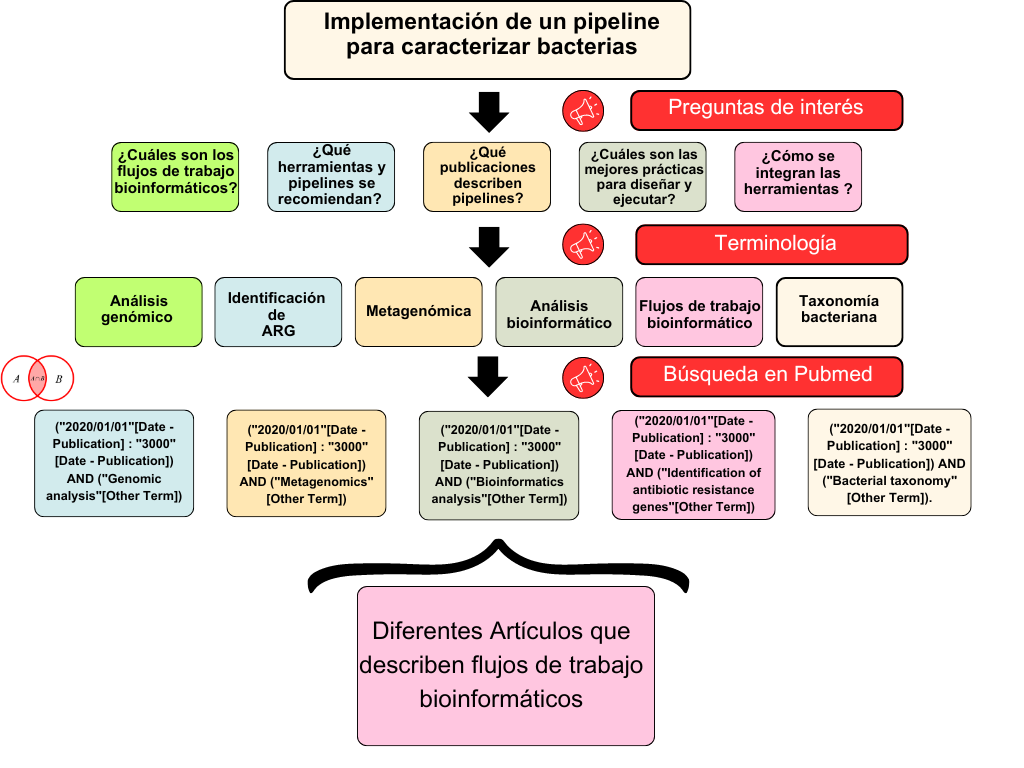
\includegraphics[scale=0.35]{anexo1.png}
    \caption{Metodología utilizada en la búsqueda bibliográfica (\emph{elaboración propia}).} 
    \label{fig:metodologiaBiblio}
\end{figure}

\newpage
\subsection{Anexo 2: Resultados del análisis taxonómico del caso de estudio \emph{elabaración propia}.}

\begin{longtable}{|p{2cm}|p{2.5cm}|p{2.5cm}|p{2.5cm}|p{1.5cm}|p{3cm}|}
    \caption{Información de cobertura, lecturas, puntos de ruptura, y taxonomía (elaboración propia).} \label{tab:coverage_info} \\
    \hline
    \textbf{Cobertura (\%)} & \textbf{N° de lecturas} & \textbf{N° Puntos de ruptura} & \textbf{ID Taxón} & \textbf{Rango} & \textbf{Taxonomía} \\
    \hline
    \endfirsthead
    
    \multicolumn{6}{c}{\tablename\ \thetable\ -- \textit{Continúa desde la página anterior}} \\
    \hline
    \textbf{Cobertura (\%)} & \textbf{N° de lecturas} & \textbf{N° Puntos de ruptura} & \textbf{ID Taxón} & \textbf{Rango} & \textbf{Taxonomía} \\
    \hline
    \endhead
    
    \hline \multicolumn{6}{r}{\textit{Continúa en la próxima página}} \\
    \endfoot
    
    \hline
    \endlastfoot
    
    94.87 & 37 & 37 & U & 0 & unclassified \\
    \hline
    5.13 & 2 & 0 & 1 & root & root \\
    \hline
    5.13 & 2 & 0 & 10239 &  & Viruses \\
    \hline
    5.13 & 2 & 0 & 2731341 & 1 & Duplodnaviria \\
    \hline
    5.13 & 2 & 0 & 2731360 & K & Heunggongvirae \\
    \hline
    5.13 & 2 & 0 & 2731618 & P & Uroviricota \\
    \hline
    5.13 & 2 & 0 & 2731619 & C & Caudoviricetes \\
    \hline
    2.56 & 1 & 0 & 2946167 & F & Peduoviridae \\
    \hline
    2.56 & 1 & 0 & 2948951 & G & Wadgaonvirus \\
    \hline
    2.56 & 1 & 0 & 2956672 & S & Wadgaonvirus wv5004651 \\
    \hline
    2.56 & 1 & 1 & 2716351 & S1 & Escherichia phage 500465-1 \\
    \hline
    2.56 & 1 & 0 & 2843442 & G & Radostvirus \\
    \hline
    2.56 & 1 & 0 & 2844247 & S & Radostvirus ev099 \\
    \hline
    2.56 & 1 & 1 & 2847061 & S1 & Escherichia phage ev099 \\
    \hline
\end{longtable}



\newpage
\subsection{Anexo 3: Resultados de la anotación funcional del caso de estudio \emph{elabaración propia}.}


\begin{longtable}{|p{1.5cm}|p{3cm}|p{5cm}|p{4cm}|}
    \caption{Resultados de la anotación funcional (elaboración propia).} \label{tab:func_annotation} \\
    \hline
    \textbf{ORF} & \textbf{Rango de Nucleótidos} & \textbf{Descripción del Producto Proteico} & \textbf{Resultados BLAST} \\
    \hline
    \endfirsthead

    \multicolumn{4}{c}{\tablename\ \thetable\ -- \textit{Continúa desde la página anterior}} \\
    \hline
    \textbf{ORF} & \textbf{Rango de Nucleótidos} & \textbf{Descripción del Producto Proteico} & \textbf{Resultados BLAST} \\
    \hline
    \endhead

    \hline \multicolumn{4}{r}{\textit{Continúa en la próxima página}} \\
    \endfoot

    \hline
    \endlastfoot

    ORF1 & 553-642 & unnamed protein product & 0 hits found \\
    \hline
    ORF2 & 113-673 & unnamed protein product & 0 hits found \\
    \hline
    ORF3 & 686-787 & unnamed protein product, partial & 0 hits found \\
    \hline
    ORF4 & 432-539 & unnamed protein product & 0 hits found \\
    \hline
    ORF5 & 402-232 & unnamed protein product & 0 hits found \\
    \hline
    ORF6 & 554-429 & unnamed protein product & 0 hits found \\
    \hline
    ORF7 & 571-47 & unnamed protein product & 0 hits found \\
    \hline
\end{longtable}


\newpage
\subsection{Anexo 4: Resultados del análisis de llamado de variantes \emph{elabaración propia}.}


\begin{longtable}{|l|l|p{8cm}|r|}
    \caption{Resultados del análisis de llamado de variantes (elaboración propia).} \label{tabla-variantes} \\
    
    \hline
    \textbf{Categoría} & \textbf{ID} & \textbf{Descripción} & \textbf{Valor} \\
    \hline
    \endfirsthead
    
    \hline
    \textbf{Categoría} & \textbf{ID} & \textbf{Descripción} & \textbf{Valor} \\
    \hline
    \endhead
    
    \hline \multicolumn{4}{|r|}{\textit{Continúa en la siguiente página}} \\ \hline
    \endfoot
    
    \hline
    \endlastfoot
    
    Número de muestras & SN & number of samples & 1 \\
    \hline
    Número de registros & SN & number of records & 90 \\
    \hline
    Número de no-ALTs & SN & number of no-ALTs & 0 \\
    \hline
    Número de SNPs & SN & number of SNPs & 90 \\
    \hline
    Número de MNPs & SN & number of MNPs & 0 \\
    \hline
    Número de indels & SN & number of indels & 0 \\
    \hline
    Número de otros & SN & number of others & 0 \\
    \hline
    Sitios multialélicos & SN & number of multiallelic sites & 0 \\
    \hline
    Sitios multialélicos SNP & SN & number of multiallelic SNP sites & 0 \\
    \hline
    Transiciones (ts) & TSTV & number of transitions & 61 \\
    \hline
    Transversiones (tv) & TSTV & number of transversions & 29 \\
    \hline
    Ratio ts/tv & TSTV & transitions/transversions ratio & 2.10 \\
    \hline
    Conteo de alelos & SiS & allele count & 1 \\
    \hline
    Número de SNPs (SiS) & SiS & number of SNPs & 90 \\
    \hline
    Transiciones (SiS) & SiS & number of transitions & 61 \\
    \hline
    Transversiones (SiS) & SiS & number of transversions & 29 \\
    \hline
    Número de indels (SiS) & SiS & number of indels & 0 \\
    \hline
    Consistente con repetición & SiS & repeat-consistent & 0 \\
    \hline
    Inconsistente con repetición & SiS & repeat-inconsistent & 0 \\
    \hline
    No aplicable (SiS) & SiS & not applicable & 0 \\
    \hline
    Frecuencia de alelo & AF & allele frequency & 0.000000 \\
    \hline
    Número de SNPs (AF) & AF & number of SNPs & 90 \\
    \hline
    Transiciones (AF) & AF & number of transitions & 61 \\
    \hline
    Transversiones (AF) & AF & number of transversions & 29 \\
    \hline
    Número de indels (AF) & AF & number of indels & 0 \\
    \hline
    Calidad media & QUAL & Quality & 30.4 \\
    \hline
    Número de SNPs (QUAL) & QUAL & number of SNPs & 90 \\
    \hline
    Transiciones (QUAL) & QUAL & number of transitions (1st ALT) & 61 \\
    \hline
    Transversiones (QUAL) & QUAL & number of transversions (1st ALT) & 29 \\
    \hline
    Tipos de Sustitución & ST & $A > C $ & 9 \\
    \hline
    Tipos de Sustitución & ST & $A > G $ & 13 \\
    \hline
    Tipos de Sustitución & ST & $ A > T $ & 4 \\
    \hline
    Tipos de Sustitución & ST & $ C > A $ & 1 \\
    \hline
    Tipos de Sustitución & ST & $ C > G $ & 2 \\
    \hline
    Tipos de Sustitución & ST & $ C > T $ & 17 \\
    \hline
    Tipos de Sustitución & ST & $ G > A $ & 13 \\
    \hline
    Tipos de Sustitución & ST & $ G > C $ & 2 \\
    \hline
    Tipos de Sustitución & ST & $ G > T $ & 2 \\
    \hline
    Tipos de Sustitución & ST & $ T > A $ & 6 \\
    \hline
    Tipos de Sustitución & ST & $ T > C $ & 18 \\
    \hline
    Tipos de Sustitución & ST & $ T > G $  & 3 \\
    \hline
    
\end{longtable}



\clearpage
\singlespacing % reduce el espacio entre citas
\bibliographystyle{ieeetr} % Estilo de citación, cambia como se escribe al final y como aparecen las citas en texto
\bibliography{main.bbl} % Las referencias están en un archivo aparte

\end{document}